\documentclass[journal,12pt,twocolumn]{IEEEtran}
%
\usepackage{setspace}
\usepackage{gensymb}
%\doublespacing
\singlespacing

%\usepackage{graphicx}
%\usepackage{amssymb}
%\usepackage{relsize}
\usepackage[cmex10]{amsmath}
%\usepackage{amsthm}
%\interdisplaylinepenalty=2500
%\savesymbol{iint}
%\usepackage{txfonts}
%\restoresymbol{TXF}{iint}
%\usepackage{wasysym}
\usepackage{amsthm}
%\usepackage{iithtlc}
\usepackage{mathrsfs}
\usepackage{txfonts}
\usepackage{stfloats}
\usepackage{bm}
\usepackage{cite}
\usepackage{cases}
\usepackage{subfig}
%\usepackage{xtab}
\usepackage{longtable}
\usepackage{multirow}
%\usepackage{algorithm}
%\usepackage{algpseudocode}
\usepackage{enumitem}
\usepackage{mathtools}
\usepackage{tikz}
\usepackage{circuitikz}
\usepackage{verbatim}
\usepackage{tfrupee}
\usepackage[breaklinks=true]{hyperref}
%\usepackage{stmaryrd}
\usepackage{tkz-euclide} % loads  TikZ and tkz-base
\usetkzobj{all}
\usepackage{listings}
    \usepackage{color}                                            %%
    \usepackage{array}                                            %%
    \usepackage{longtable}                                        %%
    \usepackage{calc}                                             %%
    \usepackage{multirow}                                         %%
    \usepackage{hhline}                                           %%
    \usepackage{ifthen}                                           %%
  %optionally (for landscape tables embedded in another document): %%
    \usepackage{lscape}     
\usepackage{multicol}
\usepackage{chngcntr}
%\usepackage{enumerate}

%\usepackage{wasysym}
%\newcounter{MYtempeqncnt}
\DeclareMathOperator*{\Res}{Res}
%\renewcommand{\baselinestretch}{2}
\renewcommand\thesection{\arabic{section}}
\renewcommand\thesubsection{\thesection.\arabic{subsection}}
\renewcommand\thesubsubsection{\thesubsection.\arabic{subsubsection}}

\renewcommand\thesectiondis{\arabic{section}}
\renewcommand\thesubsectiondis{\thesectiondis.\arabic{subsection}}
\renewcommand\thesubsubsectiondis{\thesubsectiondis.\arabic{subsubsection}}

% correct bad hyphenation here
\hyphenation{op-tical net-works semi-conduc-tor}
\def\inputGnumericTable{}                                 %%

\lstset{
%language=C,
frame=single, 
breaklines=true,
columns=fullflexible
}
%\lstset{
%language=tex,
%frame=single, 
%breaklines=true
%}

\begin{document}
%


\newtheorem{theorem}{Theorem}[section]
\newtheorem{problem}{Problem}
\newtheorem{proposition}{Proposition}[section]
\newtheorem{lemma}{Lemma}[section]
\newtheorem{corollary}[theorem]{Corollary}
\newtheorem{example}{Example}[section]
\newtheorem{definition}[problem]{Definition}
%\newtheorem{thm}{Theorem}[section] 
%\newtheorem{defn}[thm]{Definition}
%\newtheorem{algorithm}{Algorithm}[section]
%\newtheorem{cor}{Corollary}
\newcommand{\BEQA}{\begin{eqnarray}}
\newcommand{\EEQA}{\end{eqnarray}}
\newcommand{\define}{\stackrel{\triangle}{=}}

\bibliographystyle{IEEEtran}
%\bibliographystyle{ieeetr}


\providecommand{\mbf}{\mathbf}
\providecommand{\pr}[1]{\ensuremath{\Pr\left(#1\right)}}
\providecommand{\qfunc}[1]{\ensuremath{Q\left(#1\right)}}
\providecommand{\sbrak}[1]{\ensuremath{{}\left[#1\right]}}
\providecommand{\lsbrak}[1]{\ensuremath{{}\left[#1\right.}}
\providecommand{\rsbrak}[1]{\ensuremath{{}\left.#1\right]}}
\providecommand{\brak}[1]{\ensuremath{\left(#1\right)}}
\providecommand{\lbrak}[1]{\ensuremath{\left(#1\right.}}
\providecommand{\rbrak}[1]{\ensuremath{\left.#1\right)}}
\providecommand{\cbrak}[1]{\ensuremath{\left\{#1\right\}}}
\providecommand{\lcbrak}[1]{\ensuremath{\left\{#1\right.}}
\providecommand{\rcbrak}[1]{\ensuremath{\left.#1\right\}}}
\theoremstyle{remark}
\newtheorem{rem}{Remark}
\newcommand{\sgn}{\mathop{\mathrm{sgn}}}
\providecommand{\abs}[1]{\left\vert#1\right\vert}
\providecommand{\res}[1]{\Res\displaylimits_{#1}} 
\providecommand{\norm}[1]{\left\lVert#1\right\rVert}
%\providecommand{\norm}[1]{\lVert#1\rVert}
\providecommand{\mtx}[1]{\mathbf{#1}}
\providecommand{\mean}[1]{E\left[ #1 \right]}
\providecommand{\fourier}{\overset{\mathcal{F}}{ \rightleftharpoons}}
%\providecommand{\hilbert}{\overset{\mathcal{H}}{ \rightleftharpoons}}
\providecommand{\system}{\overset{\mathcal{H}}{ \longleftrightarrow}}
	%\newcommand{\solution}[2]{\textbf{Solution:}{#1}}
\newcommand{\solution}{\noindent \textbf{Solution: }}
\newcommand{\cosec}{\,\text{cosec}\,}
\providecommand{\dec}[2]{\ensuremath{\overset{#1}{\underset{#2}{\gtrless}}}}
\newcommand{\myvec}[1]{\ensuremath{\begin{pmatrix}#1\end{pmatrix}}}
\newcommand{\mydet}[1]{\ensuremath{\begin{vmatrix}#1\end{vmatrix}}}
%\numberwithin{equation}{section}
\numberwithin{equation}{subsection}
%\numberwithin{problem}{section}
%\numberwithin{definition}{section}
\makeatletter
\@addtoreset{figure}{problem}
\makeatother

\let\StandardTheFigure\thefigure
\let\vec\mathbf
%\renewcommand{\thefigure}{\theproblem.\arabic{figure}}
\renewcommand{\thefigure}{\theproblem}
%\setlist[enumerate,1]{before=\renewcommand\theequation{\theenumi.\arabic{equation}}
%\counterwithin{equation}{enumi}


%\renewcommand{\theequation}{\arabic{subsection}.\arabic{equation}}

\def\putbox#1#2#3{\makebox[0in][l]{\makebox[#1][l]{}\raisebox{\baselineskip}[0in][0in]{\raisebox{#2}[0in][0in]{#3}}}}
     \def\rightbox#1{\makebox[0in][r]{#1}}
     \def\centbox#1{\makebox[0in]{#1}}
     \def\topbox#1{\raisebox{-\baselineskip}[0in][0in]{#1}}
     \def\midbox#1{\raisebox{-0.5\baselineskip}[0in][0in]{#1}}

\vspace{3cm}

\title{
%	\logo{
Control Systems
%	}
}
\author{ G V V Sharma$^{*}$% <-this % stops a space
	\thanks{*The author is with the Department
		of Electrical Engineering, Indian Institute of Technology, Hyderabad
		502285 India e-mail:  gadepall@iith.ac.in. All content in this manual is released under GNU GPL.  Free and open source.}
	
}	
%\title{
%	\logo{Matrix Analysis through Octave}{\begin{center}\includegraphics[scale=.24]{tlc}\end{center}}{}{HAMDSP}
%}


% paper title
% can use linebreaks \\ within to get better formatting as desired
%\title{Matrix Analysis through Octave}
%
%
% author names and IEEE memberships
% note positions of commas and nonbreaking spaces ( ~ ) LaTeX will not break
% a structure at a ~ so this keeps an author's name from being broken across
% two lines.
% use \thanks{} to gain access to the first footnote area
% a separate \thanks must be used for each paragraph as LaTeX2e's \thanks
% was not built to handle multiple paragraphs
%

%\author{<-this % stops a space
%\thanks{}}
%}
% note the % following the last \IEEEmembership and also \thanks - 
% these prevent an unwanted space from occurring between the last author name
% and the end of the author line. i.e., if you had this:
% 
% \author{....lastname \thanks{...} \thanks{...} }
%                     ^------------^------------^----Do not want these spaces!
%
% a space would be appended to the last name and could cause every name on that
% line to be shifted left slightly. This is one of those "LaTeX things". For
% instance, "\textbf{A} \textbf{B}" will typeset as "A B" not "AB". To get
% "AB" then you have to do: "\textbf{A}\textbf{B}"
% \thanks is no different in this regard, so shield the last } of each \thanks
% that ends a line with a % and do not let a space in before the next \thanks.
% Spaces after \IEEEmembership other than the last one are OK (and needed) as
% you are supposed to have spaces between the names. For what it is worth,
% this is a minor point as most people would not even notice if the said evil
% space somehow managed to creep in.



% The paper headers
%\markboth{Journal of \LaTeX\ Class Files,~Vol.~6, No.~1, January~2007}%
%{Shell \MakeLowercase{\textit{et al.}}: Bare Demo of IEEEtran.cls for Journals}
% The only time the second header will appear is for the odd numbered pages
% after the title page when using the twoside option.
% 
% *** Note that you probably will NOT want to include the author's ***
% *** name in the headers of peer review papers.                   ***
% You can use \ifCLASSOPTIONpeerreview for conditional compilation here if
% you desire.




% If you want to put a publisher's ID mark on the page you can do it like
% this:
%\IEEEpubid{0000--0000/00\$00.00~\copyright~2007 IEEE}
% Remember, if you use this you must call \IEEEpubidadjcol in the second
% column for its text to clear the IEEEpubid mark.



% make the title area
\maketitle

\newpage

\tableofcontents

\bigskip

\renewcommand{\thefigure}{\theenumi}
\renewcommand{\thetable}{\theenumi}
%\renewcommand{\theequation}{\theenumi}

%\begin{abstract}
%%\boldmath
%In this letter, an algorithm for evaluating the exact analytical bit error rate  (BER)  for the piecewise linear (PL) combiner for  multiple relays is presented. Previous results were available only for upto three relays. The algorithm is unique in the sense that  the actual mathematical expressions, that are prohibitively large, need not be explicitly obtained. The diversity gain due to multiple relays is shown through plots of the analytical BER, well supported by simulations. 
%
%\end{abstract}
% IEEEtran.cls defaults to using nonbold math in the Abstract.
% This preserves the distinction between vectors and scalars. However,
% if the journal you are submitting to favors bold math in the abstract,
% then you can use LaTeX's standard command \boldmath at the very start
% of the abstract to achieve this. Many IEEE journals frown on math
% in the abstract anyway.

% Note that keywords are not normally used for peerreview papers.
%\begin{IEEEkeywords}
%Cooperative diversity, decode and forward, piecewise linear
%\end{IEEEkeywords}



% For peer review papers, you can put extra information on the cover
% page as needed:
% \ifCLASSOPTIONpeerreview
% \begin{center} \bfseries EDICS Category: 3-BBND \end{center}
% \fi
%
% For peerreview papers, this IEEEtran command inserts a page break and
% creates the second title. It will be ignored for other modes.
%\IEEEpeerreviewmaketitle

\begin{abstract}
This manual is an introduction to control systems based on GATE problems.Links to sample Python codes are available in the text.  
\end{abstract}
Download python codes using 
\begin{lstlisting}
svn co https://github.com/gadepall/school/trunk/control/codes
\end{lstlisting}

\section{Bode Plot}
\subsection{Introduction}
%%%%%%%%%%%%%%%%%%%%%%%%%%%%%%%%%%%%%%%%%%%%%%%%%%%%%%%%%%%%%%%%%%%%%%
%%                                                                  %%
%%  This is the header of a LaTeX2e file exported from Gnumeric.    %%
%%                                                                  %%
%%  This file can be compiled as it stands or included in another   %%
%%  LaTeX document. The table is based on the longtable package so  %%
%%  the longtable options (headers, footers...) can be set in the   %%
%%  preamble section below (see PRAMBLE).                           %%
%%                                                                  %%
%%  To include the file in another, the following two lines must be %%
%%  in the including file:                                          %%
%%        \def\inputGnumericTable{}                                 %%
%%  at the beginning of the file and:                               %%
%%        \input{name-of-this-file.tex}                             %%
%%  where the table is to be placed. Note also that the including   %%
%%  file must use the following packages for the table to be        %%
%%  rendered correctly:                                             %%
%%    \usepackage[latin1]{inputenc}                                 %%
%%    \usepackage{color}                                            %%
%%    \usepackage{array}                                            %%
%%    \usepackage{longtable}                                        %%
%%    \usepackage{calc}                                             %%
%%    \usepackage{multirow}                                         %%
%%    \usepackage{hhline}                                           %%
%%    \usepackage{ifthen}                                           %%
%%  optionally (for landscape tables embedded in another document): %%
%%    \usepackage{lscape}                                           %%
%%                                                                  %%
%%%%%%%%%%%%%%%%%%%%%%%%%%%%%%%%%%%%%%%%%%%%%%%%%%%%%%%%%%%%%%%%%%%%%%



%%  This section checks if we are begin input into another file or  %%
%%  the file will be compiled alone. First use a macro taken from   %%
%%  the TeXbook ex 7.7 (suggestion of Han-Wen Nienhuys).            %%
\def\ifundefined#1{\expandafter\ifx\csname#1\endcsname\relax}


%%  Check for the \def token for inputed files. If it is not        %%
%%  defined, the file will be processed as a standalone and the     %%
%%  preamble will be used.                                          %%
\ifundefined{inputGnumericTable}

%%  We must be able to close or not the document at the end.        %%
	\def\gnumericTableEnd{\end{document}}


%%%%%%%%%%%%%%%%%%%%%%%%%%%%%%%%%%%%%%%%%%%%%%%%%%%%%%%%%%%%%%%%%%%%%%
%%                                                                  %%
%%  This is the PREAMBLE. Change these values to get the right      %%
%%  paper size and other niceties.                                  %%
%%                                                                  %%
%%%%%%%%%%%%%%%%%%%%%%%%%%%%%%%%%%%%%%%%%%%%%%%%%%%%%%%%%%%%%%%%%%%%%%

	\documentclass[12pt%
			  %,landscape%
                    ]{report}
       \usepackage[latin1]{inputenc}
       \usepackage{fullpage}
       \usepackage{color}
       \usepackage{array}
       \usepackage{longtable}
       \usepackage{calc}
       \usepackage{multirow}
       \usepackage{hhline}
       \usepackage{ifthen}

	\begin{document}


%%  End of the preamble for the standalone. The next section is for %%
%%  documents which are included into other LaTeX2e files.          %%
\else

%%  We are not a stand alone document. For a regular table, we will %%
%%  have no preamble and only define the closing to mean nothing.   %%
    \def\gnumericTableEnd{}

%%  If we want landscape mode in an embedded document, comment out  %%
%%  the line above and uncomment the two below. The table will      %%
%%  begin on a new page and run in landscape mode.                  %%
%       \def\gnumericTableEnd{\end{landscape}}
%       \begin{landscape}


%%  End of the else clause for this file being \input.              %%
\fi

%%%%%%%%%%%%%%%%%%%%%%%%%%%%%%%%%%%%%%%%%%%%%%%%%%%%%%%%%%%%%%%%%%%%%%
%%                                                                  %%
%%  The rest is the gnumeric table, except for the closing          %%
%%  statement. Changes below will alter the table's appearance.     %%
%%                                                                  %%
%%%%%%%%%%%%%%%%%%%%%%%%%%%%%%%%%%%%%%%%%%%%%%%%%%%%%%%%%%%%%%%%%%%%%%

\providecommand{\gnumericmathit}[1]{#1} 
%%  Uncomment the next line if you would like your numbers to be in %%
%%  italics if they are italizised in the gnumeric table.           %%
%\renewcommand{\gnumericmathit}[1]{\mathit{#1}}
\providecommand{\gnumericPB}[1]%
{\let\gnumericTemp=\\#1\let\\=\gnumericTemp\hspace{0pt}}
 \ifundefined{gnumericTableWidthDefined}
        \newlength{\gnumericTableWidth}
        \newlength{\gnumericTableWidthComplete}
        \newlength{\gnumericMultiRowLength}
        \global\def\gnumericTableWidthDefined{}
 \fi
%% The following setting protects this code from babel shorthands.  %%
 \ifthenelse{\isundefined{\languageshorthands}}{}{\languageshorthands{english}}
%%  The default table format retains the relative column widths of  %%
%%  gnumeric. They can easily be changed to c, r or l. In that case %%
%%  you may want to comment out the next line and uncomment the one %%
%%  thereafter                                                      %%
\providecommand\gnumbox{\makebox[0pt]}
%%\providecommand\gnumbox[1][]{\makebox}

%% to adjust positions in multirow situations                       %%
\setlength{\bigstrutjot}{\jot}
\setlength{\extrarowheight}{\doublerulesep}

%%  The \setlongtables command keeps column widths the same across  %%
%%  pages. Simply comment out next line for varying column widths.  %%
\setlongtables

\setlength\gnumericTableWidth{%
	30pt+%
	38pt+%
	28pt+%
	28pt+%
0pt}
\def\gumericNumCols{4}
\setlength\gnumericTableWidthComplete{\gnumericTableWidth+%
         \tabcolsep*\gumericNumCols*2+\arrayrulewidth*\gumericNumCols}
\ifthenelse{\lengthtest{\gnumericTableWidthComplete > \linewidth}}%
         {\def\gnumericScale{\ratio{\linewidth-%
                        \tabcolsep*\gumericNumCols*2-%
                        \arrayrulewidth*\gumericNumCols}%
{\gnumericTableWidth}}}%
{\def\gnumericScale{1}}

%%%%%%%%%%%%%%%%%%%%%%%%%%%%%%%%%%%%%%%%%%%%%%%%%%%%%%%%%%%%%%%%%%%%%%
%%                                                                  %%
%% The following are the widths of the various columns. We are      %%
%% defining them here because then they are easier to change.       %%
%% Depending on the cell formats we may use them more than once.    %%
%%                                                                  %%
%%%%%%%%%%%%%%%%%%%%%%%%%%%%%%%%%%%%%%%%%%%%%%%%%%%%%%%%%%%%%%%%%%%%%%

\ifthenelse{\isundefined{\gnumericColA}}{\newlength{\gnumericColA}}{}\settowidth{\gnumericColA}{\begin{tabular}{@{}p{30pt*\gnumericScale}@{}}x\end{tabular}}
\ifthenelse{\isundefined{\gnumericColB}}{\newlength{\gnumericColB}}{}\settowidth{\gnumericColB}{\begin{tabular}{@{}p{38pt*\gnumericScale}@{}}x\end{tabular}}
\ifthenelse{\isundefined{\gnumericColC}}{\newlength{\gnumericColC}}{}\settowidth{\gnumericColC}{\begin{tabular}{@{}p{28pt*\gnumericScale}@{}}x\end{tabular}}
\ifthenelse{\isundefined{\gnumericColD}}{\newlength{\gnumericColD}}{}\settowidth{\gnumericColD}{\begin{tabular}{@{}p{28pt*\gnumericScale}@{}}x\end{tabular}}

\begin{tabular}[c]{%
	b{\gnumericColA}%
	b{\gnumericColB}%
	b{\gnumericColC}%
	b{\gnumericColD}%
	}

%%%%%%%%%%%%%%%%%%%%%%%%%%%%%%%%%%%%%%%%%%%%%%%%%%%%%%%%%%%%%%%%%%%%%%
%%  The longtable options. (Caption, headers... see Goosens, p.124) %%
%	\caption{The Table Caption.}             \\	%
% \hline	% Across the top of the table.
%%  The rest of these options are table rows which are placed on    %%
%%  the first, last or every page. Use \multicolumn if you want.    %%

%%  Header for the first page.                                      %%
%	\multicolumn{4}{c}{The First Header} \\ \hline 
%	\multicolumn{1}{c}{colTag}	%Column 1
%	&\multicolumn{1}{c}{colTag}	%Column 2
%	&\multicolumn{1}{c}{colTag}	%Column 3
%	&\multicolumn{1}{c}{colTag}	\\ \hline %Last column
%	\endfirsthead

%%  The running header definition.                                  %%
%	\hline
%	\multicolumn{4}{l}{\ldots\small\slshape continued} \\ \hline
%	\multicolumn{1}{c}{colTag}	%Column 1
%	&\multicolumn{1}{c}{colTag}	%Column 2
%	&\multicolumn{1}{c}{colTag}	%Column 3
%	&\multicolumn{1}{c}{colTag}	\\ \hline %Last column
%	\endhead

%%  The running footer definition.                                  %%
%	\hline
%	\multicolumn{4}{r}{\small\slshape continued\ldots} \\
%	\endfoot

%%  The ending footer definition.                                   %%
%	\multicolumn{4}{c}{That's all folks} \\ \hline 
%	\endlastfoot
%%%%%%%%%%%%%%%%%%%%%%%%%%%%%%%%%%%%%%%%%%%%%%%%%%%%%%%%%%%%%%%%%%%%%%

\hhline{|-|-|-|-}
	 \multicolumn{1}{|p{\gnumericColA}|}%
	{\gnumericPB{\centering}\gnumbox{\textbf{$f$ (Hz)}}}
	&\multicolumn{1}{p{\gnumericColB}|}%
	{\gnumericPB{\centering}\gnumbox{\textbf{$\Delta\brak{\nabla G(f)}$}}}
	&\multicolumn{1}{p{\gnumericColC}|}%
	{\gnumericPB{\centering}\gnumbox{\textbf{Pole}}}
	&\multicolumn{1}{p{\gnumericColD}|}%
	{\gnumericPB{\centering}\gnumbox{\textbf{Zero}}}
\\
\hhline{|----|}
	 \multicolumn{1}{|p{\gnumericColA}|}%
	{\gnumericPB{\centering}\gnumbox{$10^1$}}
	&\multicolumn{1}{p{\gnumericColB}|}%
	{\gnumericPB{\centering}\gnumbox{-20}}
	&\multicolumn{1}{p{\gnumericColC}|}%
	{\gnumericPB{\centering}\gnumbox{1}}
	&\multicolumn{1}{p{\gnumericColD}|}%
	{\gnumericPB{\centering}\gnumbox{0}}
\\
\hhline{|----|}
	 \multicolumn{1}{|p{\gnumericColA}|}%
	{\gnumericPB{\centering}\gnumbox{$10^2$}}
	&\multicolumn{1}{p{\gnumericColB}|}%
	{\gnumericPB{\centering}\gnumbox{-40}}
	&\multicolumn{1}{p{\gnumericColC}|}%
	{\gnumericPB{\centering}\gnumbox{2}}
	&\multicolumn{1}{p{\gnumericColD}|}%
	{\gnumericPB{\centering}\gnumbox{0}}
\\
\hhline{|----|}
	 \multicolumn{1}{|p{\gnumericColA}|}%
	{\gnumericPB{\centering}\gnumbox{$10^3$}}
	&\multicolumn{1}{p{\gnumericColB}|}%
	{\gnumericPB{\centering}\gnumbox{20}}
	&\multicolumn{1}{p{\gnumericColC}|}%
	{\gnumericPB{\centering}\gnumbox{0}}
	&\multicolumn{1}{p{\gnumericColD}|}%
	{\gnumericPB{\centering}\gnumbox{1}}
\\
\hhline{|----|}
	 \multicolumn{1}{|p{\gnumericColA}|}%
	{\gnumericPB{\centering}\gnumbox{$10^4$}}
	&\multicolumn{1}{p{\gnumericColB}|}%
	{\gnumericPB{\centering}\gnumbox{40}}
	&\multicolumn{1}{p{\gnumericColC}|}%
	{\gnumericPB{\centering}\gnumbox{0}}
	&\multicolumn{1}{p{\gnumericColD}|}%
	{\gnumericPB{\centering}\gnumbox{2}}
\\
\hhline{|----|}
	 \multicolumn{1}{|p{\gnumericColA}|}%
	{\gnumericPB{\centering}\gnumbox{$10^5$}}
	&\multicolumn{1}{p{\gnumericColB}|}%
	{\gnumericPB{\centering}\gnumbox{-40}}
	&\multicolumn{1}{p{\gnumericColC}|}%
	{\gnumericPB{\centering}\gnumbox{2}}
	&\multicolumn{1}{p{\gnumericColD}|}%
	{\gnumericPB{\centering}\gnumbox{0}}
\\
\hhline{|----|}
	 \multicolumn{1}{|p{\gnumericColA}|}%
	{\gnumericPB{\centering}\gnumbox{$10^6$}}
	&\multicolumn{1}{p{\gnumericColB}|}%
	{\gnumericPB{\centering}\gnumbox{-20}}
	&\multicolumn{1}{p{\gnumericColC}|}%
	{\gnumericPB{\centering}\gnumbox{1}}
	&\multicolumn{1}{p{\gnumericColD}|}%
	{\gnumericPB{\centering}\gnumbox{0}}
\\
\hhline{|----|}
	 \multicolumn{1}{|p{\gnumericColA}|}%
	{\gnumericPB{\centering}\gnumbox{\textbf{Total}}}
	&\multicolumn{1}{p{\gnumericColB}|}%
	{}
	&\multicolumn{1}{p{\gnumericColC}|}%
	{\gnumericPB{\centering}\gnumbox{\textbf{6}}}
	&\multicolumn{1}{p{\gnumericColD}|}%
	{\gnumericPB{\centering}\gnumbox{\textbf{3}}}
\\
\hhline{|-|-|-|-|}
\end{tabular}

\ifthenelse{\isundefined{\languageshorthands}}{}{\languageshorthands{\languagename}}
\gnumericTableEnd

\subsection{Example}
\begin{enumerate}[label=\thesubsection.\arabic*.,ref=\thesubsection.\theenumi]
\numberwithin{equation}{enumi} 
\item 
The asymptotic Bode magnitude plot of  minimum phase transfer function
G(s) is show below.\\
\begin{figure}[htp]
	\centering
	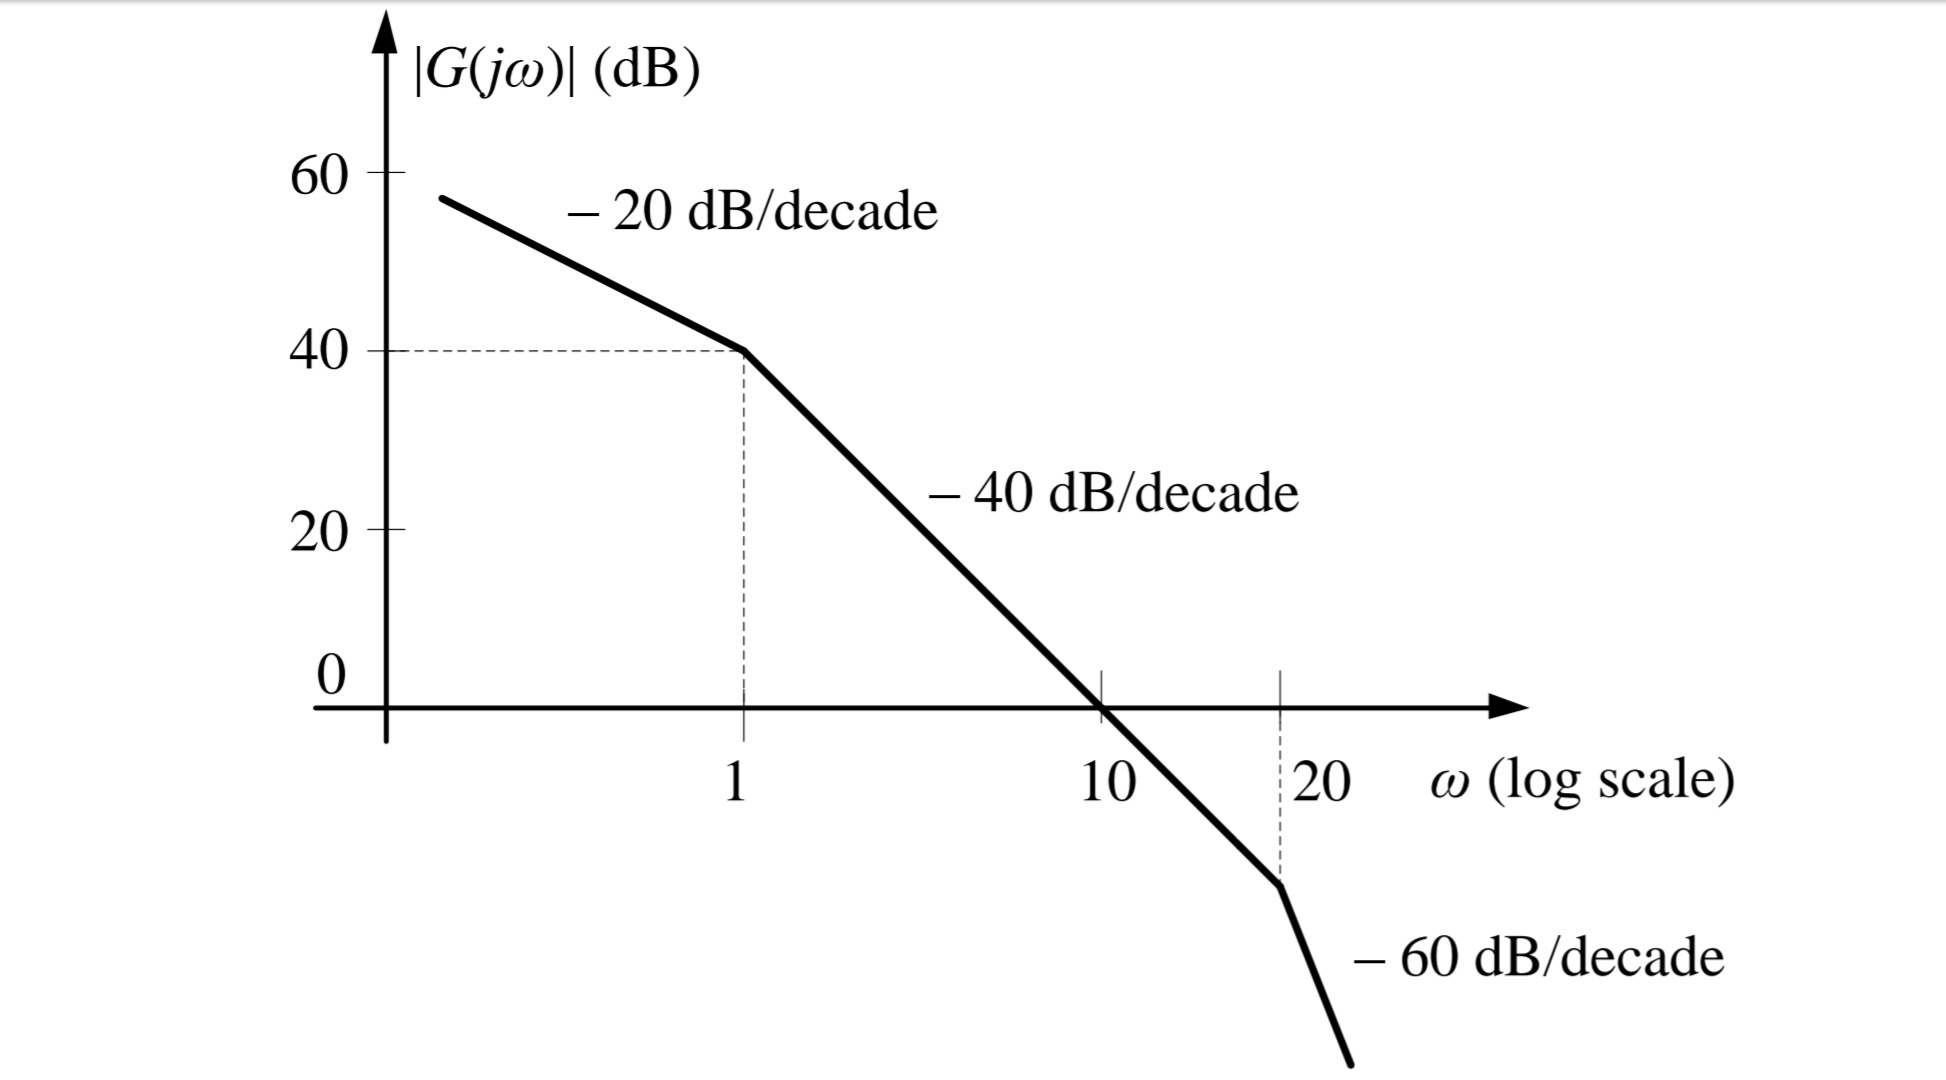
\includegraphics[width=1 \columnwidth]{./figs/ee18btech11009/pppp.eps}
	\caption{}
	\label{fig:galaxy}
\end{figure} 
\item Verify if the transfer function G(s) has 3 poles and one zero.
\item  Verify if at very high frequency $(\omega \to \infty)$, the phase angle $ \angle G(j\omega)=-3\pi/2$
\solution

Since, each pole corresponds to -20 dB/decade  
and each zero corresponds to +20 dB/decade.\\
Therefore, from the given Bode plot we can get the Transfer equation,
\begin{align}
G(s) = \frac{k}{s(1+s)(20+s)}
\end{align}

Now, from the Transfer equation we can conclude that,
there are three poles (0, -1 and -20 ) and no zeros.\\

$\therefore$ Statement 1 is false  ..........(1)\\ \\

%------------------------------------------------

\textbf{Calculating phase:}\\ \\
Since we know that,\\
phase $ \phi $ is the sum of all the phases corresponding to each pole and zero.\\
phase corresponding to pole is =  
\begin{align}
-tan^{-1}( \frac{imaginary}{real})
\end{align} 
phase corresponding to zero is =
\begin{align}
 tan^{-1}( \frac{imaginary}{real})
 \end{align} 
%------------------------------------------------
Now take,
\begin{align}
 s = j\omega
  \end{align} 
  \begin{align}
 \Rightarrow  G(j\omega) =  \frac{k}{j\omega(1+j\omega)(20+j\omega)}
 \end{align} 
Therefore, 
\begin{align}
 \phi =  -tan^{-1}( {\frac{\omega}{0}}) - tan^{-1}(\omega) - tan^{-1}( \frac{\omega}{20})
 \end{align} 
 \begin{align}
  \phi =  - 90^\circ - tan^{-1}(\omega) - tan^{-1}( \frac{\omega}{20})
  \end{align} 
  \begin{align}
  \because \omega \to \infty
 \end{align} 
 \begin{align}
   \phi =   - 90^\circ - 90^\circ - 90^\circ
   \end{align} 
   \begin{align}
 \phi = -270^\circ
 \end{align} 
 \begin{align}
 \phi = -3\pi/2 
 \end{align} 
 $\therefore$ Statement 2 is true ........(2)\\
 thus, from (1) and (2) option (B) is correct.
 \\
 \\
 \item
%\begin{flushleft}

 \end{enumerate}

\section{Stability}
\subsection{Second order System}
\begin{enumerate}[label=\thesection.\arabic*.,ref=\thesection.\theenumi]
\numberwithin{equation}{enumi}
\item
Consider the following second order system with the transfer function
\begin{align}
G(s) = \frac{1}{1+2s+s^2}
\end{align}
Is the system stable? 
\\
\solution The poles of 
\begin{align}
G(s) = \frac{1}{1+2s+s^2}
\end{align}
are at 
\begin{align}
s = -1
\end{align}
i.e.,  the left half of s-plane.  Hence the system is stable.
\item Find and sketch the step response $c(t)$ of the system.
\\
\solution 
For step-response, we take input as unit-step function u(t)
\begin{align}
C(s) &= U(s).G(s) = \sbrak{\frac{1}{s}} \sbrak{\frac{1}{1+2s+s^2}}
\\
&= \frac{1}{s(1+s)^2}
\\
&= \frac{1}{s} - \frac{1}{(1+s)} - \frac{1}{(1+s)^2}
\end{align}
%
Taking the inverse Laplace transform,
%
\begin{align}
c(t) &= L^{-1} \sbrak{ \frac{1}{s}} - L^{-1}\sbrak{\frac{1}{1+s}} - L^{-1}\sbrak{\frac{1}{(1+s)^2}} 
\\
&= \brak{1 - e^{-t} - te^{-t}}  u(t)
\label{eq:sec_order_op}
\end{align}
%
The following code plots $c(t)$ in Fig. \ref{fig:sec_order}
\begin{lstlisting}
codes/ee18btech11002/plot.py
\end{lstlisting}
\begin{figure}
\centering
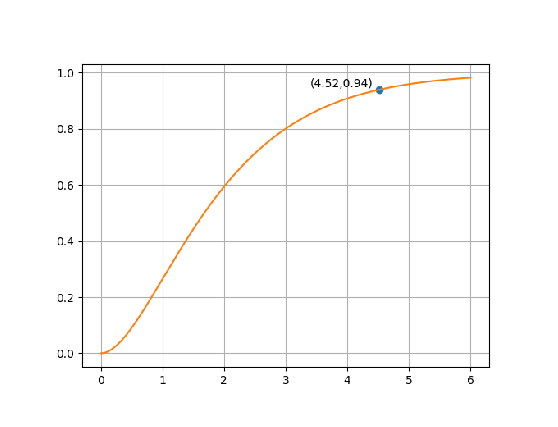
\includegraphics[width=\columnwidth]{./figs/ee18btech11002.eps}
\caption{}
\label{fig:sec_order}
\end{figure}
\item Find the steady state response of the system using the final value theorem.  Verify using 
\ref{eq:sec_order_op}
\\
\solution 
To know the steady response value of c(t), using final value theorem,
\begin{align}
\lim_{t\to\infty} c(t) = \lim_{s\to 0} sC(s) 
\end{align}
We get
\begin{align}
\lim_{s\to 0} s \brak{\frac{1}{s}}\brak{\frac{1}{1+s+s^2}} = \frac{1}{1+0+0} = 1
\end{align}
Using \ref{eq:sec_order_op}, 
\begin{align}
\lim_{t\to\infty} c(t) &=\lim_{t\to\infty}\brak{1 - e^{-t} - te^{-t}}  u(t) 
\\
&=(1-0-0) = 1 
\end{align}
%
\item Find the time taken for the system output c(t) to reach 94\% of its steady state value.
\\
\solution 
Now, 94\% of 1 is 0.94, so we should now solve for a positive t such that
\begin{align}
1 - e^{-t} - te^{-t} = 0.94
\end{align}
The following code 
%
\begin{lstlisting}
codes/ee18btech11002/solution.py
\end{lstlisting}
%\lstinputlisting{./}
provides the necessary solution as 
%the attached code gives us the solution for the equation
%and t turns out to be
\begin{align}
 t = 4.5228
\end{align}

\end{enumerate}

\section{Routh Hurwitz Criterion}
\subsection{Marginal Stability}
\begin{enumerate}[label=\thesection.\arabic*.,ref=\thesection.\theenumi]
\numberwithin{equation}{enumi}

\item
Consider a unity feedback system as shown in Fig.  \ref{fig:ee18btech11005}, with an integral compensator $\frac{k}{s}$ and open-loop transfer function
\begin{align}
G(s) = \frac{1}{s^2+3s+2}
\end{align}
where k greater than 0. 
%
Find its closed loop transfer function.
\begin{figure}[!ht]
	\begin{center}
		
		\resizebox{\columnwidth}{!}{\begin{enumerate}[label=\thesection.\arabic*.,ref=\thesection.\theenumi]
\numberwithin{equation}{enumi}

\item
Consider a unity feedback system as shown in Fig.  \ref{fig:ee18btech11005}, with an integral compensator $\frac{k}{s}$ and open-loop transfer function
\begin{align}
G(s) = \frac{1}{s^2+3s+2}
\end{align}
where k greater than 0. 
%
Find its closed loop transfer function.
\begin{figure}[!ht]
	\begin{center}
		
		\resizebox{\columnwidth}{!}{\begin{enumerate}[label=\thesection.\arabic*.,ref=\thesection.\theenumi]
\numberwithin{equation}{enumi}

\item
Consider a unity feedback system as shown in Fig.  \ref{fig:ee18btech11005}, with an integral compensator $\frac{k}{s}$ and open-loop transfer function
\begin{align}
G(s) = \frac{1}{s^2+3s+2}
\end{align}
where k greater than 0. 
%
Find its closed loop transfer function.
\begin{figure}[!ht]
	\begin{center}
		
		\resizebox{\columnwidth}{!}{\input{./figs/ee18btech11005.tex}}
	\end{center}
\caption{}
\label{fig:ee18btech11005}
\end{figure}

\solution $\because H(s) = 1$ in Fig.  \ref{fig:ee18btech11005}, due to unity feedback,   the transfer function is given by
\begin{align}
\frac{Y(s)}{X(s)} &= \frac{G(s)}{1+G(s)H(s)}
\\
\implies T(s) &= \frac{k}{s^3+3s^2+2s}
\end{align}
%
\item Find the {\em characteristic} equation for $G(s)$.
\\
\solution The characteristic equation is
\begin{align}
\label{eq:routh_char_eq}
 1 + G(s)H(s) &= 0 
\\
\implies 1 + \sbrak{\frac{k}{s^3+3s^2+2s}} &= 0
\\
\text{or, } s^3+3s^2+2s+k &= 0
\end{align}
\item Using the tabular method for the Routh hurwitz criterion, find $k > 0$ for which there are two poles of unity feedback system on j${\omega}$ axis.
%
\\
\solution 
This criterion is based on arranging the coefficients of characteristic equation into an array called Routh array.
For any characteristic equation 
\begin{multline}
q(s) = a_0s^n+a_1s^{n-1}+.....+a_{n-1}s+a_n = 0
\end{multline}
the Routh array can be constructed as 
 
\begin{align}
\mydet{s^n\\s^{n-1}\\s^{n-2} \\ \vdots}
 \mydet{a_0 & a_2 & a_4 & \cdots \\
a_1 & a_3 & a_5 & \cdots  \\
b_1 & b_2 & b_3 & \cdots \\
\vdots & \vdots & \vdots & \ddots &\vdots 
 \cdots \\}
\end{align}
%
 where
 \begin{align}
 b_1 =\frac{ a_1a_2-a_0a_3}{a_1}  
 \\
 b_2 =\frac{ a_1a_4-a_0a_5}{a_1} 
 \\
 c_1=\frac{ b_1a_3-a_1b_2}{b_1} 
\\
 c_2=\frac{ b_1a_5-a_1b_3}{b_1}  
\end{align}
For poles to lie on imaginary axis any one entire row of hurwitz matrix should be zero.
Constructing the routh array for the characteristic equation obtained in \ref{eq:routh_char_eq},
%
\begin{align}
 s^3+3s^2+2s+k = 0
\end{align}
%
\begin{align}
\mydet{s^3\\s^2\\s^1 \\ s^0}
\mydet{1 & 2 \\ 3 & k \\  \frac{6-k}{3} & 0\\ k & 0}
\end{align}
For poles on $\j \omega$ axis any one of the row should be zero.
%
\begin{align}
\therefore \frac{6-k}{3} &= 0 \text{ or } k = 0
\\
\implies k &= 6 \quad \because k > 0
\end{align}
\item Repeat the above using the determinant method.
\\
\solution The {\em Routh matrix} can be expressed as
\begin{align}
\vec{R} = \myvec{a_0 & a_2 & a_4 & \cdots \\
a_1 & a_3 & a_5 & \cdots  \\
 0 & a_0 & a_2\cdots \\
 0 & a_1 & a_3 \cdots\\
\vdots & \vdots & \vdots & \ddots &\vdots 
\cdots \\}
\end{align}
and the corresponding Routh determinants are
\begin{align}
D_1 &= |a_0|
\\
D_2 &= 
\mydet{
a_0 & a_2 
\\ 
a_1 & a_3
} 
\\
D_3 &=\mydet{
a_0 & a_2 & a_4 
\\ a_1 & a_3 & a_5 
\\ 0 & a_0 & a_2}
\\
\dots
\end{align}
If at least any one of the Determinents are zero then the poles lie on imaginary axes.  From \eqref{eq:routh_char_eq},
%
\begin{align}
D_1 &= 1 \ne 0
\\
D2 &= \mydet{
1 & 2 \\ 3 & k } 
&= k-6 =0 \implies k = 6
\end{align}
%
\item Verify your answer using a python code for both the determinant method as well as the tabular method.
\\
\solution 
The following code 
%
\begin{lstlisting}
codes/ee18btech11005/ee18btech11005.py
\end{lstlisting}
%
provides the necessary soution.
\begin{itemize}
\item  For the system to be stable all coefficients should lie on left half of s-plane. Because if any pole is in right half of s-plane then there will be a component in output that increases without bound,causing system to be unstable.
All the coefficients in the characteristic equation should be positive.This is necessary condition but not sufficient.Because it may have poles on right half of s plane.
Poles are the roots of the characteristic equation.
    \item A system is stable if all of its characteristic modes go to finite value as t goes to infinity.It is possible only if all the poles are on the left half of s plane.
    The characteristic equation should have negative roots only. So the first column should always be greater than zero.That means no sign changes.
    \item A system is unstable if its characteristic modes are not bounded. Then the characteristic equation will also have roots in the right side of s-plane.That means it has sign changes.
    \end{itemize}

\end{enumerate}


}
	\end{center}
\caption{}
\label{fig:ee18btech11005}
\end{figure}

\solution $\because H(s) = 1$ in Fig.  \ref{fig:ee18btech11005}, due to unity feedback,   the transfer function is given by
\begin{align}
\frac{Y(s)}{X(s)} &= \frac{G(s)}{1+G(s)H(s)}
\\
\implies T(s) &= \frac{k}{s^3+3s^2+2s}
\end{align}
%
\item Find the {\em characteristic} equation for $G(s)$.
\\
\solution The characteristic equation is
\begin{align}
\label{eq:routh_char_eq}
 1 + G(s)H(s) &= 0 
\\
\implies 1 + \sbrak{\frac{k}{s^3+3s^2+2s}} &= 0
\\
\text{or, } s^3+3s^2+2s+k &= 0
\end{align}
\item Using the tabular method for the Routh hurwitz criterion, find $k > 0$ for which there are two poles of unity feedback system on j${\omega}$ axis.
%
\\
\solution 
This criterion is based on arranging the coefficients of characteristic equation into an array called Routh array.
For any characteristic equation 
\begin{multline}
q(s) = a_0s^n+a_1s^{n-1}+.....+a_{n-1}s+a_n = 0
\end{multline}
the Routh array can be constructed as 
 
\begin{align}
\mydet{s^n\\s^{n-1}\\s^{n-2} \\ \vdots}
 \mydet{a_0 & a_2 & a_4 & \cdots \\
a_1 & a_3 & a_5 & \cdots  \\
b_1 & b_2 & b_3 & \cdots \\
\vdots & \vdots & \vdots & \ddots &\vdots 
 \cdots \\}
\end{align}
%
 where
 \begin{align}
 b_1 =\frac{ a_1a_2-a_0a_3}{a_1}  
 \\
 b_2 =\frac{ a_1a_4-a_0a_5}{a_1} 
 \\
 c_1=\frac{ b_1a_3-a_1b_2}{b_1} 
\\
 c_2=\frac{ b_1a_5-a_1b_3}{b_1}  
\end{align}
For poles to lie on imaginary axis any one entire row of hurwitz matrix should be zero.
Constructing the routh array for the characteristic equation obtained in \ref{eq:routh_char_eq},
%
\begin{align}
 s^3+3s^2+2s+k = 0
\end{align}
%
\begin{align}
\mydet{s^3\\s^2\\s^1 \\ s^0}
\mydet{1 & 2 \\ 3 & k \\  \frac{6-k}{3} & 0\\ k & 0}
\end{align}
For poles on $\j \omega$ axis any one of the row should be zero.
%
\begin{align}
\therefore \frac{6-k}{3} &= 0 \text{ or } k = 0
\\
\implies k &= 6 \quad \because k > 0
\end{align}
\item Repeat the above using the determinant method.
\\
\solution The {\em Routh matrix} can be expressed as
\begin{align}
\vec{R} = \myvec{a_0 & a_2 & a_4 & \cdots \\
a_1 & a_3 & a_5 & \cdots  \\
 0 & a_0 & a_2\cdots \\
 0 & a_1 & a_3 \cdots\\
\vdots & \vdots & \vdots & \ddots &\vdots 
\cdots \\}
\end{align}
and the corresponding Routh determinants are
\begin{align}
D_1 &= |a_0|
\\
D_2 &= 
\mydet{
a_0 & a_2 
\\ 
a_1 & a_3
} 
\\
D_3 &=\mydet{
a_0 & a_2 & a_4 
\\ a_1 & a_3 & a_5 
\\ 0 & a_0 & a_2}
\\
\dots
\end{align}
If at least any one of the Determinents are zero then the poles lie on imaginary axes.  From \eqref{eq:routh_char_eq},
%
\begin{align}
D_1 &= 1 \ne 0
\\
D2 &= \mydet{
1 & 2 \\ 3 & k } 
&= k-6 =0 \implies k = 6
\end{align}
%
\item Verify your answer using a python code for both the determinant method as well as the tabular method.
\\
\solution 
The following code 
%
\begin{lstlisting}
codes/ee18btech11005/ee18btech11005.py
\end{lstlisting}
%
provides the necessary soution.
\begin{itemize}
\item  For the system to be stable all coefficients should lie on left half of s-plane. Because if any pole is in right half of s-plane then there will be a component in output that increases without bound,causing system to be unstable.
All the coefficients in the characteristic equation should be positive.This is necessary condition but not sufficient.Because it may have poles on right half of s plane.
Poles are the roots of the characteristic equation.
    \item A system is stable if all of its characteristic modes go to finite value as t goes to infinity.It is possible only if all the poles are on the left half of s plane.
    The characteristic equation should have negative roots only. So the first column should always be greater than zero.That means no sign changes.
    \item A system is unstable if its characteristic modes are not bounded. Then the characteristic equation will also have roots in the right side of s-plane.That means it has sign changes.
    \end{itemize}

\end{enumerate}


}
	\end{center}
\caption{}
\label{fig:ee18btech11005}
\end{figure}

\solution $\because H(s) = 1$ in Fig.  \ref{fig:ee18btech11005}, due to unity feedback,   the transfer function is given by
\begin{align}
\frac{Y(s)}{X(s)} &= \frac{G(s)}{1+G(s)H(s)}
\\
\implies T(s) &= \frac{k}{s^3+3s^2+2s}
\end{align}
%
\item Find the {\em characteristic} equation for $G(s)$.
\\
\solution The characteristic equation is
\begin{align}
\label{eq:routh_char_eq}
 1 + G(s)H(s) &= 0 
\\
\implies 1 + \sbrak{\frac{k}{s^3+3s^2+2s}} &= 0
\\
\text{or, } s^3+3s^2+2s+k &= 0
\end{align}
\item Using the tabular method for the Routh hurwitz criterion, find $k > 0$ for which there are two poles of unity feedback system on j${\omega}$ axis.
%
\\
\solution 
This criterion is based on arranging the coefficients of characteristic equation into an array called Routh array.
For any characteristic equation 
\begin{multline}
q(s) = a_0s^n+a_1s^{n-1}+.....+a_{n-1}s+a_n = 0
\end{multline}
the Routh array can be constructed as 
 
\begin{align}
\mydet{s^n\\s^{n-1}\\s^{n-2} \\ \vdots}
 \mydet{a_0 & a_2 & a_4 & \cdots \\
a_1 & a_3 & a_5 & \cdots  \\
b_1 & b_2 & b_3 & \cdots \\
\vdots & \vdots & \vdots & \ddots &\vdots 
 \cdots \\}
\end{align}
%
 where
 \begin{align}
 b_1 =\frac{ a_1a_2-a_0a_3}{a_1}  
 \\
 b_2 =\frac{ a_1a_4-a_0a_5}{a_1} 
 \\
 c_1=\frac{ b_1a_3-a_1b_2}{b_1} 
\\
 c_2=\frac{ b_1a_5-a_1b_3}{b_1}  
\end{align}
For poles to lie on imaginary axis any one entire row of hurwitz matrix should be zero.
Constructing the routh array for the characteristic equation obtained in \ref{eq:routh_char_eq},
%
\begin{align}
 s^3+3s^2+2s+k = 0
\end{align}
%
\begin{align}
\mydet{s^3\\s^2\\s^1 \\ s^0}
\mydet{1 & 2 \\ 3 & k \\  \frac{6-k}{3} & 0\\ k & 0}
\end{align}
For poles on $\j \omega$ axis any one of the row should be zero.
%
\begin{align}
\therefore \frac{6-k}{3} &= 0 \text{ or } k = 0
\\
\implies k &= 6 \quad \because k > 0
\end{align}
\item Repeat the above using the determinant method.
\\
\solution The {\em Routh matrix} can be expressed as
\begin{align}
\vec{R} = \myvec{a_0 & a_2 & a_4 & \cdots \\
a_1 & a_3 & a_5 & \cdots  \\
 0 & a_0 & a_2\cdots \\
 0 & a_1 & a_3 \cdots\\
\vdots & \vdots & \vdots & \ddots &\vdots 
\cdots \\}
\end{align}
and the corresponding Routh determinants are
\begin{align}
D_1 &= |a_0|
\\
D_2 &= 
\mydet{
a_0 & a_2 
\\ 
a_1 & a_3
} 
\\
D_3 &=\mydet{
a_0 & a_2 & a_4 
\\ a_1 & a_3 & a_5 
\\ 0 & a_0 & a_2}
\\
\dots
\end{align}
If at least any one of the Determinents are zero then the poles lie on imaginary axes.  From \eqref{eq:routh_char_eq},
%
\begin{align}
D_1 &= 1 \ne 0
\\
D2 &= \mydet{
1 & 2 \\ 3 & k } 
&= k-6 =0 \implies k = 6
\end{align}
%
\item Verify your answer using a python code for both the determinant method as well as the tabular method.
\\
\solution 
The following code 
%
\begin{lstlisting}
codes/ee18btech11005/ee18btech11005.py
\end{lstlisting}
%
provides the necessary soution.
\begin{itemize}
\item  For the system to be stable all coefficients should lie on left half of s-plane. Because if any pole is in right half of s-plane then there will be a component in output that increases without bound,causing system to be unstable.
All the coefficients in the characteristic equation should be positive.This is necessary condition but not sufficient.Because it may have poles on right half of s plane.
Poles are the roots of the characteristic equation.
    \item A system is stable if all of its characteristic modes go to finite value as t goes to infinity.It is possible only if all the poles are on the left half of s plane.
    The characteristic equation should have negative roots only. So the first column should always be greater than zero.That means no sign changes.
    \item A system is unstable if its characteristic modes are not bounded. Then the characteristic equation will also have roots in the right side of s-plane.That means it has sign changes.
    \end{itemize}

\end{enumerate}



\subsection{Stability}
\begin{enumerate}[label=\thesubsection.\arabic*.,ref=\thesubsection.\theenumi]
\numberwithin{equation}{enumi}
\item 
The characteristic equation of linear time invariant system is given by
\begin{align} 
\nabla(s)=s^4+3s^3+3s^2+s+k=0
\end{align}
Find the condition for the system to be BIBO stable using the Routh Array.

\textbf{solution}
\begin{align}
\nabla(s)=s^4+3s^3+3s^2+s+k=0
\end{align}

The Routh hurwitz criterion:-
\bigskip
\begin{align}
\mydet{s^4\\s^3\\s^2\\s^1 \\ s^0}
\mydet{1 & 3 & k \\ 3 & 1 & 0\\  \frac{8}{3}& k & 0\\ \frac{\frac{8}{3}-3k}{\frac{8}{3}} & 0 & 0\\k & 0 & 0} 
\end{align}
From the above array, the given system is stable if
\begin{align}
\begin{split}
k&>0 
\\
  \frac{\frac{8}{3}-3k}{\frac{8}{3}}&>0    
\end{split}
\\
\implies 0<k<\frac{8}{9}
\end{align}
%
\item Modify the Python code in Problem \ref{prob:ee18btech11005_python} to verify your solution by choosing two different values of $k$.
\label{prob:ee18btech11008_python}
\\
\solution 
The following code 
%
\begin{lstlisting}
codes/ee18btech11008.py
\end{lstlisting}
%
provides the necessary soution.

\end{enumerate}

\section{State-Space Model}
\subsection{Controllability and Observabiity}
\begin{enumerate}[label=\thesection.\arabic*.,ref=\thesection.\theenumi]
\numberwithin{equation}{enumi}
\item State the general model of a state space system specifying the dimensions of the matrices and vectors.
\\
\solution The model is given by 
\begin{align}
\dot{\vec{x}}(t)&=\vec{A}\vec{x}(t)+\vec{B}\vec{u}(t) \\
 \vec{y}(t)&=\vec{C}\vec{x}(t)+\vec{D} \vec{u}(t)
\end{align}
%
with parameters listed in Table \ref{table:ee18btech11004}.
%
\begin{table}[!ht]
\centering
\begin{enumerate}[label=\thesection.\arabic*.,ref=\thesection.\theenumi]
\numberwithin{equation}{enumi}
\item State the general model of a state space system specifying the dimensions of the matrices and vectors.
\\
\solution The model is given by 
\begin{align}
\dot{\vec{x}}(t)&=\vec{A}\vec{x}(t)+\vec{B}\vec{u}(t) \\
 \vec{y}(t)&=\vec{C}\vec{x}(t)+\vec{D} \vec{u}(t)
\end{align}
%
with parameters listed in Table \ref{table:ee18btech11004}.
%
\begin{table}[!ht]
\centering
\begin{enumerate}[label=\thesection.\arabic*.,ref=\thesection.\theenumi]
\numberwithin{equation}{enumi}
\item State the general model of a state space system specifying the dimensions of the matrices and vectors.
\\
\solution The model is given by 
\begin{align}
\dot{\vec{x}}(t)&=\vec{A}\vec{x}(t)+\vec{B}\vec{u}(t) \\
 \vec{y}(t)&=\vec{C}\vec{x}(t)+\vec{D} \vec{u}(t)
\end{align}
%
with parameters listed in Table \ref{table:ee18btech11004}.
%
\begin{table}[!ht]
\centering
\input{./tables/ee18btech11004.tex}
\caption{}
\label{table:ee18btech11004}
\end{table}
\item Find the transfer function $\vec{H}(s)$ for the general system.
\\
\solution 
Taking Laplace transform on both sides we have the following equations
\begin{align}
s\vec{I}X(s)-x(0)= \vec{A}X(s)+ \vec{B}U(s)\\
(s\vec{I}-\vec{A})X(s)= \vec{B}U(s)+ x(0)\\
X(s)={(s\vec{I}-\vec{A})^{-1}}\vec{B} U(s)+ (s\vec{I}-\vec{A})^{-1}x(0)
\label{eq:x_init}
\end{align}
and
\begin{align}
Y(s)= \vec{C}X(s)+D\vec{I}U(s)
\end{align}
Substituting from \eqref{eq:x_init} in the above,
%
\begin{multline}
Y(s)=( \vec{C}{(s\vec{I}-\vec{A})^{-1}}\vec{B}+D\vec{I}) U(s) 
\\
+ \vec{C}(s\vec{I}-\vec{A})^{-1}x(0)
\end{multline}
%
\item Find $H(s)$ for a SISO (single input single output) system.
\\
\solution
\begin{align}
H(s)= {\frac{Y(s)}{U(s)}}= C{(sI-A)^{-1}}B+DI
\end{align}

\item Given 
\begin{align}
H(s)&=\frac{1}{s^3+3s^2+2s+1}
\\
D&=0
\\
\vec{B}&= \myvec{0\\0\\1}
\end{align}
%
 find $\vec{A}$ and $\vec{C}$ such that the state-space realization is in {\em controllable canonical form}.
\\
\solution 
\begin{align} 
\because {\frac{Y(s)}{U(s)}}= \frac{Y(s)}{V(s)} \times \frac{V(s)}{U(s)},
\end{align}
letting
\begin{align}
 {\frac{Y(s)}{V(s)}}= 1, 
\end{align}
results in 
\begin{align}
{\frac{U(s)}{V(s)}}={s^3 + 3s^2+2s + 1}
\end{align}

giving
\begin{align}
U(s)= s^3 V(s) + 3s^2 V(s)+2sV(s) + V(s)
\end{align}

so equation 0.1.13 can be written as
\begin{align}
\myvec{sV(s)\\s^2V(s)\\s^3V(s)}
=
\myvec{0&1&0\\0&0&1\\-1&-2&-3}\myvec{V(s)\\s(s)\\s^2V(s)}
+
\myvec{0\\0\\1}  U
\end{align}
So 
\begin{align}
\vec{A}=\myvec{0&1&0\\0&0&1\\-1&-2&-3}
\end{align}

\begin{align}
Y=X_{1}(s)
=\myvec{1&0&0} \myvec{V(s)\\sV(s)\\s^2V(s)}
\end{align}
\begin{align}
\vec{C}=\myvec{1&0&0}
\end{align}

\item Obtain $\vec{A}$ and $\vec{C}$ so that the state-space realization in in {\em observable canonical form}.
\\
\solution  Given that
\begin{align}
H(s)&=\frac{1}{s^3+3s^2+2s+1}
\end{align}
\begin{align}
\frac{Y(s)}{U(s)}=\frac{1}{s^3+3s^2+2s+1} \\
Y(s) \times (s^3+3s^2+2s+1) = U(s)
\end{align}
\begin{align}
s^3Y(s)+3s^2Y(s)+2sY(s)+Y(s)=U(s)\\
s^3Y(s)=U(s)-3s^2Y(s)-2sY(s)-Y(s)\\
Y(s)=-3s^{-1}Y(s)-2s^{-2}Y(s)+s^{-3}(U(s)-Y(s))
\end{align}
\\ let $Y=aU+X_{1}$
\\ by comparing with equation 1.5.6 we get a=0 and
\begin{align}
Y=X_{1}
\end{align}
inverse laplace transform of above equation is 
\begin{align}
y=x_{1}
\end{align}
so from above equation 1.5.6 and 1.5.7
\begin{align}
X_{1}=-3s^{-1}Y(s)-2s^{-2}Y(s)+s^{-3}(U(s)-Y(s))\\
sX_{1}=-3Y(s)-2s^{-1}Y(s)+s^{-2}(U(s)-Y(s)) 
\end{align}
inverse laplace transform of above equation 
\begin{align}
\dot{x_{1}}=-3y+x_{2}
\end{align} 
where
\begin{align}
X_{2}=-2s^{-1}Y(s)+s^{-2}(U(s)-Y(s))\\
sX_{2}=-2Y(s)+s^{-1}(U(s)-Y(s))
\end{align} 
inverse laplace transform of above equation 
\begin{align}
\dot{x_{2}}=-2y+x_{3}
\end{align}
where
\begin{align}
X_{3}=s^{-1}(U(s)-Y(s))\\
sX_{3}=U(s)-Y(s)
\end{align} 
inverse laplace transform of above equation 
\begin{align}
\dot{x_{3}}=u-y
\end{align}
so we get four equations which are
\begin{align}
y=x_{1}\\
\dot{x_{1}}=-3y+x_{2}\\
\dot{x_{2}}=-2y+x_{3}\\
\dot{x_{3}}=u-y
\end{align} 
sub $ y=x_{1}$ in 1.5.19,1.5.20,1.5.21 we get
\begin{align}
 y=x_{1}\\
\dot{x_{1}}=-3x_{1}+x_{2}\\
\dot{x_{2}}=-2x_{1}+x_{3}\\
\dot{x_{3}}=u-x_{1}
\end{align} 
so above equations can be written as
\begin{align}
\myvec{\dot{x_{1}}\\\dot{x_{2}}\\\dot{x_{3}})}
=
\myvec{-3&1&0\\-2&0&1\\-1&0&0}\myvec{x_{1}\\x_{2}\\x_{3}}
+
\myvec{0\\0\\1}  U
\end{align}
So 
\begin{align}
\vec{A}=\myvec{-3&1&0\\-2&0&1\\-1&0&0}
\end{align}
\begin{align}
y=x_{1}
=\myvec{1&0&0} \myvec{x_{1}\\x_{2}\\x_{3}}
\end{align}
\begin{align}
\vec{C}=\myvec{1&0&0}
\end{align}


\item Find the eigenvaues of $\vec{A}$ and the poles of $H(s)$ using a python code.
\\
\solution The following code 
%
\begin{lstlisting}
codes/ee18btech11004.py
\end{lstlisting}
gives the necessary values.  The roots are the same as the eigenvalues.
%
\item Theoretically, show that eigenvaues of $\vec{A}$ are the poles of  $H(s)$.
\solution 
\\ as we know tthat  the characteristic equation is det(sI-A) 
\\\begin{align}
\vec{sI-A}=
\myvec{s&0&0\\0&s&0\\0&0&s}
-
\myvec{0&1&0\\0&0&1\\-1&-2&-3}
=\myvec{s&-1&0\\0&s&-1\\1&2&s+3}
\end{align}
\\therfore
\begin{align}
det(sI-A)=s(s^2+3s+2)+1(1)=s^3+3s^2+2s+1
\end{align} 
\\so from equation 1.6.2 we can see that charcteristic equation is equal to the denominator of the transefer function
\end{enumerate}


\caption{}
\label{table:ee18btech11004}
\end{table}
\item Find the transfer function $\vec{H}(s)$ for the general system.
\\
\solution 
Taking Laplace transform on both sides we have the following equations
\begin{align}
s\vec{I}X(s)-x(0)= \vec{A}X(s)+ \vec{B}U(s)\\
(s\vec{I}-\vec{A})X(s)= \vec{B}U(s)+ x(0)\\
X(s)={(s\vec{I}-\vec{A})^{-1}}\vec{B} U(s)+ (s\vec{I}-\vec{A})^{-1}x(0)
\label{eq:x_init}
\end{align}
and
\begin{align}
Y(s)= \vec{C}X(s)+D\vec{I}U(s)
\end{align}
Substituting from \eqref{eq:x_init} in the above,
%
\begin{multline}
Y(s)=( \vec{C}{(s\vec{I}-\vec{A})^{-1}}\vec{B}+D\vec{I}) U(s) 
\\
+ \vec{C}(s\vec{I}-\vec{A})^{-1}x(0)
\end{multline}
%
\item Find $H(s)$ for a SISO (single input single output) system.
\\
\solution
\begin{align}
H(s)= {\frac{Y(s)}{U(s)}}= C{(sI-A)^{-1}}B+DI
\end{align}

\item Given 
\begin{align}
H(s)&=\frac{1}{s^3+3s^2+2s+1}
\\
D&=0
\\
\vec{B}&= \myvec{0\\0\\1}
\end{align}
%
 find $\vec{A}$ and $\vec{C}$ such that the state-space realization is in {\em controllable canonical form}.
\\
\solution 
\begin{align} 
\because {\frac{Y(s)}{U(s)}}= \frac{Y(s)}{V(s)} \times \frac{V(s)}{U(s)},
\end{align}
letting
\begin{align}
 {\frac{Y(s)}{V(s)}}= 1, 
\end{align}
results in 
\begin{align}
{\frac{U(s)}{V(s)}}={s^3 + 3s^2+2s + 1}
\end{align}

giving
\begin{align}
U(s)= s^3 V(s) + 3s^2 V(s)+2sV(s) + V(s)
\end{align}

so equation 0.1.13 can be written as
\begin{align}
\myvec{sV(s)\\s^2V(s)\\s^3V(s)}
=
\myvec{0&1&0\\0&0&1\\-1&-2&-3}\myvec{V(s)\\s(s)\\s^2V(s)}
+
\myvec{0\\0\\1}  U
\end{align}
So 
\begin{align}
\vec{A}=\myvec{0&1&0\\0&0&1\\-1&-2&-3}
\end{align}

\begin{align}
Y=X_{1}(s)
=\myvec{1&0&0} \myvec{V(s)\\sV(s)\\s^2V(s)}
\end{align}
\begin{align}
\vec{C}=\myvec{1&0&0}
\end{align}

\item Obtain $\vec{A}$ and $\vec{C}$ so that the state-space realization in in {\em observable canonical form}.
\\
\solution  Given that
\begin{align}
H(s)&=\frac{1}{s^3+3s^2+2s+1}
\end{align}
\begin{align}
\frac{Y(s)}{U(s)}=\frac{1}{s^3+3s^2+2s+1} \\
Y(s) \times (s^3+3s^2+2s+1) = U(s)
\end{align}
\begin{align}
s^3Y(s)+3s^2Y(s)+2sY(s)+Y(s)=U(s)\\
s^3Y(s)=U(s)-3s^2Y(s)-2sY(s)-Y(s)\\
Y(s)=-3s^{-1}Y(s)-2s^{-2}Y(s)+s^{-3}(U(s)-Y(s))
\end{align}
\\ let $Y=aU+X_{1}$
\\ by comparing with equation 1.5.6 we get a=0 and
\begin{align}
Y=X_{1}
\end{align}
inverse laplace transform of above equation is 
\begin{align}
y=x_{1}
\end{align}
so from above equation 1.5.6 and 1.5.7
\begin{align}
X_{1}=-3s^{-1}Y(s)-2s^{-2}Y(s)+s^{-3}(U(s)-Y(s))\\
sX_{1}=-3Y(s)-2s^{-1}Y(s)+s^{-2}(U(s)-Y(s)) 
\end{align}
inverse laplace transform of above equation 
\begin{align}
\dot{x_{1}}=-3y+x_{2}
\end{align} 
where
\begin{align}
X_{2}=-2s^{-1}Y(s)+s^{-2}(U(s)-Y(s))\\
sX_{2}=-2Y(s)+s^{-1}(U(s)-Y(s))
\end{align} 
inverse laplace transform of above equation 
\begin{align}
\dot{x_{2}}=-2y+x_{3}
\end{align}
where
\begin{align}
X_{3}=s^{-1}(U(s)-Y(s))\\
sX_{3}=U(s)-Y(s)
\end{align} 
inverse laplace transform of above equation 
\begin{align}
\dot{x_{3}}=u-y
\end{align}
so we get four equations which are
\begin{align}
y=x_{1}\\
\dot{x_{1}}=-3y+x_{2}\\
\dot{x_{2}}=-2y+x_{3}\\
\dot{x_{3}}=u-y
\end{align} 
sub $ y=x_{1}$ in 1.5.19,1.5.20,1.5.21 we get
\begin{align}
 y=x_{1}\\
\dot{x_{1}}=-3x_{1}+x_{2}\\
\dot{x_{2}}=-2x_{1}+x_{3}\\
\dot{x_{3}}=u-x_{1}
\end{align} 
so above equations can be written as
\begin{align}
\myvec{\dot{x_{1}}\\\dot{x_{2}}\\\dot{x_{3}})}
=
\myvec{-3&1&0\\-2&0&1\\-1&0&0}\myvec{x_{1}\\x_{2}\\x_{3}}
+
\myvec{0\\0\\1}  U
\end{align}
So 
\begin{align}
\vec{A}=\myvec{-3&1&0\\-2&0&1\\-1&0&0}
\end{align}
\begin{align}
y=x_{1}
=\myvec{1&0&0} \myvec{x_{1}\\x_{2}\\x_{3}}
\end{align}
\begin{align}
\vec{C}=\myvec{1&0&0}
\end{align}


\item Find the eigenvaues of $\vec{A}$ and the poles of $H(s)$ using a python code.
\\
\solution The following code 
%
\begin{lstlisting}
codes/ee18btech11004.py
\end{lstlisting}
gives the necessary values.  The roots are the same as the eigenvalues.
%
\item Theoretically, show that eigenvaues of $\vec{A}$ are the poles of  $H(s)$.
\solution 
\\ as we know tthat  the characteristic equation is det(sI-A) 
\\\begin{align}
\vec{sI-A}=
\myvec{s&0&0\\0&s&0\\0&0&s}
-
\myvec{0&1&0\\0&0&1\\-1&-2&-3}
=\myvec{s&-1&0\\0&s&-1\\1&2&s+3}
\end{align}
\\therfore
\begin{align}
det(sI-A)=s(s^2+3s+2)+1(1)=s^3+3s^2+2s+1
\end{align} 
\\so from equation 1.6.2 we can see that charcteristic equation is equal to the denominator of the transefer function
\end{enumerate}


\caption{}
\label{table:ee18btech11004}
\end{table}
\item Find the transfer function $\vec{H}(s)$ for the general system.
\\
\solution 
Taking Laplace transform on both sides we have the following equations
\begin{align}
s\vec{I}X(s)-x(0)= \vec{A}X(s)+ \vec{B}U(s)\\
(s\vec{I}-\vec{A})X(s)= \vec{B}U(s)+ x(0)\\
X(s)={(s\vec{I}-\vec{A})^{-1}}\vec{B} U(s)+ (s\vec{I}-\vec{A})^{-1}x(0)
\label{eq:x_init}
\end{align}
and
\begin{align}
Y(s)= \vec{C}X(s)+D\vec{I}U(s)
\end{align}
Substituting from \eqref{eq:x_init} in the above,
%
\begin{multline}
Y(s)=( \vec{C}{(s\vec{I}-\vec{A})^{-1}}\vec{B}+D\vec{I}) U(s) 
\\
+ \vec{C}(s\vec{I}-\vec{A})^{-1}x(0)
\end{multline}
%
\item Find $H(s)$ for a SISO (single input single output) system.
\\
\solution
\begin{align}
H(s)= {\frac{Y(s)}{U(s)}}= C{(sI-A)^{-1}}B+DI
\end{align}

\item Given 
\begin{align}
H(s)&=\frac{1}{s^3+3s^2+2s+1}
\\
D&=0
\\
\vec{B}&= \myvec{0\\0\\1}
\end{align}
%
 find $\vec{A}$ and $\vec{C}$ such that the state-space realization is in {\em controllable canonical form}.
\\
\solution 
\begin{align} 
\because {\frac{Y(s)}{U(s)}}= \frac{Y(s)}{V(s)} \times \frac{V(s)}{U(s)},
\end{align}
letting
\begin{align}
 {\frac{Y(s)}{V(s)}}= 1, 
\end{align}
results in 
\begin{align}
{\frac{U(s)}{V(s)}}={s^3 + 3s^2+2s + 1}
\end{align}

giving
\begin{align}
U(s)= s^3 V(s) + 3s^2 V(s)+2sV(s) + V(s)
\end{align}

so equation 0.1.13 can be written as
\begin{align}
\myvec{sV(s)\\s^2V(s)\\s^3V(s)}
=
\myvec{0&1&0\\0&0&1\\-1&-2&-3}\myvec{V(s)\\s(s)\\s^2V(s)}
+
\myvec{0\\0\\1}  U
\end{align}
So 
\begin{align}
\vec{A}=\myvec{0&1&0\\0&0&1\\-1&-2&-3}
\end{align}

\begin{align}
Y=X_{1}(s)
=\myvec{1&0&0} \myvec{V(s)\\sV(s)\\s^2V(s)}
\end{align}
\begin{align}
\vec{C}=\myvec{1&0&0}
\end{align}

\item Obtain $\vec{A}$ and $\vec{C}$ so that the state-space realization in in {\em observable canonical form}.
\\
\solution  Given that
\begin{align}
H(s)&=\frac{1}{s^3+3s^2+2s+1}
\end{align}
\begin{align}
\frac{Y(s)}{U(s)}=\frac{1}{s^3+3s^2+2s+1} \\
Y(s) \times (s^3+3s^2+2s+1) = U(s)
\end{align}
\begin{align}
s^3Y(s)+3s^2Y(s)+2sY(s)+Y(s)=U(s)\\
s^3Y(s)=U(s)-3s^2Y(s)-2sY(s)-Y(s)\\
Y(s)=-3s^{-1}Y(s)-2s^{-2}Y(s)+s^{-3}(U(s)-Y(s))
\end{align}
\\ let $Y=aU+X_{1}$
\\ by comparing with equation 1.5.6 we get a=0 and
\begin{align}
Y=X_{1}
\end{align}
inverse laplace transform of above equation is 
\begin{align}
y=x_{1}
\end{align}
so from above equation 1.5.6 and 1.5.7
\begin{align}
X_{1}=-3s^{-1}Y(s)-2s^{-2}Y(s)+s^{-3}(U(s)-Y(s))\\
sX_{1}=-3Y(s)-2s^{-1}Y(s)+s^{-2}(U(s)-Y(s)) 
\end{align}
inverse laplace transform of above equation 
\begin{align}
\dot{x_{1}}=-3y+x_{2}
\end{align} 
where
\begin{align}
X_{2}=-2s^{-1}Y(s)+s^{-2}(U(s)-Y(s))\\
sX_{2}=-2Y(s)+s^{-1}(U(s)-Y(s))
\end{align} 
inverse laplace transform of above equation 
\begin{align}
\dot{x_{2}}=-2y+x_{3}
\end{align}
where
\begin{align}
X_{3}=s^{-1}(U(s)-Y(s))\\
sX_{3}=U(s)-Y(s)
\end{align} 
inverse laplace transform of above equation 
\begin{align}
\dot{x_{3}}=u-y
\end{align}
so we get four equations which are
\begin{align}
y=x_{1}\\
\dot{x_{1}}=-3y+x_{2}\\
\dot{x_{2}}=-2y+x_{3}\\
\dot{x_{3}}=u-y
\end{align} 
sub $ y=x_{1}$ in 1.5.19,1.5.20,1.5.21 we get
\begin{align}
 y=x_{1}\\
\dot{x_{1}}=-3x_{1}+x_{2}\\
\dot{x_{2}}=-2x_{1}+x_{3}\\
\dot{x_{3}}=u-x_{1}
\end{align} 
so above equations can be written as
\begin{align}
\myvec{\dot{x_{1}}\\\dot{x_{2}}\\\dot{x_{3}})}
=
\myvec{-3&1&0\\-2&0&1\\-1&0&0}\myvec{x_{1}\\x_{2}\\x_{3}}
+
\myvec{0\\0\\1}  U
\end{align}
So 
\begin{align}
\vec{A}=\myvec{-3&1&0\\-2&0&1\\-1&0&0}
\end{align}
\begin{align}
y=x_{1}
=\myvec{1&0&0} \myvec{x_{1}\\x_{2}\\x_{3}}
\end{align}
\begin{align}
\vec{C}=\myvec{1&0&0}
\end{align}


\item Find the eigenvaues of $\vec{A}$ and the poles of $H(s)$ using a python code.
\\
\solution The following code 
%
\begin{lstlisting}
codes/ee18btech11004.py
\end{lstlisting}
gives the necessary values.  The roots are the same as the eigenvalues.
%
\item Theoretically, show that eigenvaues of $\vec{A}$ are the poles of  $H(s)$.
\solution 
\\ as we know tthat  the characteristic equation is det(sI-A) 
\\\begin{align}
\vec{sI-A}=
\myvec{s&0&0\\0&s&0\\0&0&s}
-
\myvec{0&1&0\\0&0&1\\-1&-2&-3}
=\myvec{s&-1&0\\0&s&-1\\1&2&s+3}
\end{align}
\\therfore
\begin{align}
det(sI-A)=s(s^2+3s+2)+1(1)=s^3+3s^2+2s+1
\end{align} 
\\so from equation 1.6.2 we can see that charcteristic equation is equal to the denominator of the transefer function
\end{enumerate}


\subsection{Second Order System}
%%%%%%%%%%%%%%%%%%%%%%%%%%%%%%%%%%%%%%%%%%%%%%%%%%%%%%%%%%%%%%%%%%%%%%
%%                                                                  %%
%%  This is the header of a LaTeX2e file exported from Gnumeric.    %%
%%                                                                  %%
%%  This file can be compiled as it stands or included in another   %%
%%  LaTeX document. The table is based on the longtable package so  %%
%%  the longtable options (headers, footers...) can be set in the   %%
%%  preamble section below (see PRAMBLE).                           %%
%%                                                                  %%
%%  To include the file in another, the following two lines must be %%
%%  in the including file:                                          %%
%%        \def\inputGnumericTable{}                                 %%
%%  at the beginning of the file and:                               %%
%%        \input{name-of-this-file.tex}                             %%
%%  where the table is to be placed. Note also that the including   %%
%%  file must use the following packages for the table to be        %%
%%  rendered correctly:                                             %%
%%    \usepackage[latin1]{inputenc}                                 %%
%%    \usepackage{color}                                            %%
%%    \usepackage{array}                                            %%
%%    \usepackage{longtable}                                        %%
%%    \usepackage{calc}                                             %%
%%    \usepackage{multirow}                                         %%
%%    \usepackage{hhline}                                           %%
%%    \usepackage{ifthen}                                           %%
%%  optionally (for landscape tables embedded in another document): %%
%%    \usepackage{lscape}                                           %%
%%                                                                  %%
%%%%%%%%%%%%%%%%%%%%%%%%%%%%%%%%%%%%%%%%%%%%%%%%%%%%%%%%%%%%%%%%%%%%%%



%%  This section checks if we are begin input into another file or  %%
%%  the file will be compiled alone. First use a macro taken from   %%
%%  the TeXbook ex 7.7 (suggestion of Han-Wen Nienhuys).            %%
\def\ifundefined#1{\expandafter\ifx\csname#1\endcsname\relax}


%%  Check for the \def token for inputed files. If it is not        %%
%%  defined, the file will be processed as a standalone and the     %%
%%  preamble will be used.                                          %%
\ifundefined{inputGnumericTable}

%%  We must be able to close or not the document at the end.        %%
	\def\gnumericTableEnd{\end{document}}


%%%%%%%%%%%%%%%%%%%%%%%%%%%%%%%%%%%%%%%%%%%%%%%%%%%%%%%%%%%%%%%%%%%%%%
%%                                                                  %%
%%  This is the PREAMBLE. Change these values to get the right      %%
%%  paper size and other niceties.                                  %%
%%                                                                  %%
%%%%%%%%%%%%%%%%%%%%%%%%%%%%%%%%%%%%%%%%%%%%%%%%%%%%%%%%%%%%%%%%%%%%%%

	\documentclass[12pt%
			  %,landscape%
                    ]{report}
       \usepackage[latin1]{inputenc}
       \usepackage{fullpage}
       \usepackage{color}
       \usepackage{array}
       \usepackage{longtable}
       \usepackage{calc}
       \usepackage{multirow}
       \usepackage{hhline}
       \usepackage{ifthen}

	\begin{document}


%%  End of the preamble for the standalone. The next section is for %%
%%  documents which are included into other LaTeX2e files.          %%
\else

%%  We are not a stand alone document. For a regular table, we will %%
%%  have no preamble and only define the closing to mean nothing.   %%
    \def\gnumericTableEnd{}

%%  If we want landscape mode in an embedded document, comment out  %%
%%  the line above and uncomment the two below. The table will      %%
%%  begin on a new page and run in landscape mode.                  %%
%       \def\gnumericTableEnd{\end{landscape}}
%       \begin{landscape}


%%  End of the else clause for this file being \input.              %%
\fi

%%%%%%%%%%%%%%%%%%%%%%%%%%%%%%%%%%%%%%%%%%%%%%%%%%%%%%%%%%%%%%%%%%%%%%
%%                                                                  %%
%%  The rest is the gnumeric table, except for the closing          %%
%%  statement. Changes below will alter the table's appearance.     %%
%%                                                                  %%
%%%%%%%%%%%%%%%%%%%%%%%%%%%%%%%%%%%%%%%%%%%%%%%%%%%%%%%%%%%%%%%%%%%%%%

\providecommand{\gnumericmathit}[1]{#1} 
%%  Uncomment the next line if you would like your numbers to be in %%
%%  italics if they are italizised in the gnumeric table.           %%
%\renewcommand{\gnumericmathit}[1]{\mathit{#1}}
\providecommand{\gnumericPB}[1]%
{\let\gnumericTemp=\\#1\let\\=\gnumericTemp\hspace{0pt}}
 \ifundefined{gnumericTableWidthDefined}
        \newlength{\gnumericTableWidth}
        \newlength{\gnumericTableWidthComplete}
        \newlength{\gnumericMultiRowLength}
        \global\def\gnumericTableWidthDefined{}
 \fi
%% The following setting protects this code from babel shorthands.  %%
 \ifthenelse{\isundefined{\languageshorthands}}{}{\languageshorthands{english}}
%%  The default table format retains the relative column widths of  %%
%%  gnumeric. They can easily be changed to c, r or l. In that case %%
%%  you may want to comment out the next line and uncomment the one %%
%%  thereafter                                                      %%
\providecommand\gnumbox{\makebox[0pt]}
%%\providecommand\gnumbox[1][]{\makebox}

%% to adjust positions in multirow situations                       %%
\setlength{\bigstrutjot}{\jot}
\setlength{\extrarowheight}{\doublerulesep}

%%  The \setlongtables command keeps column widths the same across  %%
%%  pages. Simply comment out next line for varying column widths.  %%
\setlongtables

\setlength\gnumericTableWidth{%
	70pt+%
	70pt+%
0pt}
\def\gumericNumCols{3}
\setlength\gnumericTableWidthComplete{\gnumericTableWidth+%
         \tabcolsep*\gumericNumCols*2+\arrayrulewidth*\gumericNumCols}
\ifthenelse{\lengthtest{\gnumericTableWidthComplete > \linewidth}}%
         {\def\gnumericScale{\ratio{\linewidth-%
                        \tabcolsep*\gumericNumCols*2-%
                        \arrayrulewidth*\gumericNumCols}%
{\gnumericTableWidth}}}%
{\def\gnumericScale{1}}

%%%%%%%%%%%%%%%%%%%%%%%%%%%%%%%%%%%%%%%%%%%%%%%%%%%%%%%%%%%%%%%%%%%%%%
%%                                                                  %%
%% The following are the widths of the various columns. We are      %%
%% defining them here because then they are easier to change.       %%
%% Depending on the cell formats we may use them more than once.    %%
%%                                                                  %%
%%%%%%%%%%%%%%%%%%%%%%%%%%%%%%%%%%%%%%%%%%%%%%%%%%%%%%%%%%%%%%%%%%%%%%

\ifthenelse{\isundefined{\gnumericColA}}{\newlength{\gnumericColA}}{}\settowidth{\gnumericColA}{\begin{tabular}{@{}p{70pt*\gnumericScale}@{}}x\end{tabular}}
\ifthenelse{\isundefined{\gnumericColB}}{\newlength{\gnumericColB}}{}\settowidth{\gnumericColB}{\begin{tabular}{@{}p{70pt*\gnumericScale}@{}}x\end{tabular}}

\begin{tabular}[c]{%
	b{\gnumericColA}%
	b{\gnumericColB}%
	}

%%%%%%%%%%%%%%%%%%%%%%%%%%%%%%%%%%%%%%%%%%%%%%%%%%%%%%%%%%%%%%%%%%%%%%
%%  The longtable options. (Caption, headers... see Goosens, p.124) %%
%	\caption{The Table Caption.}             \\	%
% \hline	% Across the top of the table.
%%  The rest of these options are table rows which are placed on    %%
%%  the first, last or every page. Use \multicolumn if you want.    %%

%%  Header for the first page.                                      %%
%	\multicolumn{3}{c}{The First Header} \\ \hline 
%	\multicolumn{1}{c}{colTag}	%Column 1
%	&\multicolumn{1}{c}{colTag}	%Column 2
%	&\multicolumn{1}{c}{colTag}	\\ \hline %Last column
%	\endfirsthead

%%  The running header definition.                                  %%
%	\hline
%	\multicolumn{3}{l}{\ldots\small\slshape continued} \\ \hline
%	\multicolumn{1}{c}{colTag}	%Column 1
%	&\multicolumn{1}{c}{colTag}	%Column 2
%	&\multicolumn{1}{c}{colTag}	\\ \hline %Last column
%	\endhead

%%  The running footer definition.                                  %%
%	\hline
%	\multicolumn{3}{r}{\small\slshape continued\ldots} \\
%	\endfoot

%%  The ending footer definition.                                   %%
%	\multicolumn{3}{c}{That's all folks} \\ \hline 
%	\endlastfoot
%%%%%%%%%%%%%%%%%%%%%%%%%%%%%%%%%%%%%%%%%%%%%%%%%%%%%%%%%%%%%%%%%%%%%%

\hhline{|-|-|-}
	 \multicolumn{1}{|p{\gnumericColA}|}%
	{\gnumericPB{\centering}\textbf{Damping ratio($\zeta$)}}
	&\multicolumn{1}{p{\gnumericColB}|}%
	{\gnumericPB{\centering}\textbf{Undamped natural frequency($\omega_{n}$)}}
\\
\hhline{|---|}
	 \multicolumn{1}{|p{\gnumericColA}|}%
	{\gnumericPB{\raggedright}Damping ratio basically indicates the amount of damping present in the overall system denoted by zeta, where damping is a counter force.It is a dimensionless measure describing how oscillations in a system decay after a disturbance.}
	&\multicolumn{1}{p{\gnumericColB}|}%
	{\gnumericPB{\raggedright}The frequency of oscillation of the system without damping.A system may or may not have an associated natural frequency.}
\\
\hhline{|---|}
	 \multicolumn{1}{|p{\gnumericColA}|}%
	{\gnumericPB{\centering}The damping ratio is a system parameter, denoted by $\zeta$, that can vary from undamped ($\zeta$ = 0), underdamped ($\zeta$ \textless 1) through critically damped ($\zeta$ = 1) to overdamped ($\zeta$ \textgreater 1).}
	&\multicolumn{1}{p{\gnumericColB}|}%
	{\gnumericPB{\raggedright}Only systems with $\zeta$ \textless 1 have a natural frequency $\omega$ and only in the case that $\zeta$ = 0 will the natural frequency $\omega$ = $\omega_{n}$, the undamped natural frequency.}
\\
\hhline{|-|-|-|}
\end{tabular}

\ifthenelse{\isundefined{\languageshorthands}}{}{\languageshorthands{\languagename}}
\gnumericTableEnd


\section{Nyquist Plot}
\begin{enumerate}[label=\thesection.\arabic*.,ref=\thesection.\theenumi]
\numberwithin{equation}{enumi}
\item The open loop transfer function of a unity feedback system is given by
\begin{align}
\label{eq:ee18btech11007_system}
 G(s)=\frac{\pi e^{-0.25s}}{s}
\end{align}
\item Find $\text{Re} \cbrak{G(\j \omega)}$ and $\text{Im} \cbrak{G(\j \omega)}$.
\\
\solution From \eqref{eq:ee18btech11007_system},
%
\begin{align}
G(j\omega)&=\frac{\pi}{\omega}(-\sin{0.25\omega}-j\cos{0.25\omega})
\\
\implies  \text{Re} \cbrak{G(\j \omega)}&=\frac{\pi}{\omega}(-\sin{0.25\omega}) 
\\
 \text{Im} \cbrak{G(\j \omega)}&=\frac{\pi}{\omega}(-j\cos{0.25\omega}) 
\end{align}
%
\item Sketch the Nyquist plot.
\\
\solution The Nyquist plot is a graph of $\text{Re} \cbrak{G(\j \omega)}$  vs $\text{Im} \cbrak{G(\j \omega)}$.
The following python code generates the Nyquist plot in Fig.  \ref{fig:ee18btech11007}
%
\begin{figure}[!h]
  \includegraphics[width=\columnwidth]{./figs/ee18btech11007.eps}
  \caption{}
  \label{fig:ee18btech11007}
\end{figure}
%
\item Find the point at which the Nyquist plot of G(s) passes through the negative real axis
\\
\solution  Nyquist plot cuts the negative real axis at $\omega $ for which 
\begin{align}
\angle G(\j\omega)=-\pi
\label{eq:ee18btech11007_system_neg_real}
\end{align}
From \eqref{eq:ee18btech11007_system},
\begin{align}
 G(\j\omega)&=\frac{\pi e^{-\frac{\j\omega}{4}}}{\j\omega} = \frac{\pi e^{-\j\brak{\frac{\omega}{4}+\frac{\pi}{2}}}}{\omega}
\\
\implies \angle{ G(\j\omega)} &= -\brak{\frac{\omega}{4}+\frac{\pi}{2}}
\label{eq:ee18btech11007_system_ang}
\end{align}
From \eqref{eq:ee18btech11007_system_ang} and \eqref{eq:ee18btech11007_system_neg_real}, 
\begin{align}
\frac{\omega}{4}+\frac{\pi}{2} &= \pi
\\
\implies \omega = 2\pi
\end{align}
Also, from \eqref{eq:ee18btech11007_system},
\begin{align}
\label{eq:ee18btech11007_system_mod}
\abs{ G(\j\omega)}&=\frac{\pi }{\abs{\omega}}
\\
\implies \abs{ G(\j2\pi)} &= \frac{1}{2}
\end{align}
%
\item Find the value of $P$ defined in Table \ref{table:ee18btech11007} from Fig.  \ref{fig:ee18btech11007}.
\begin{table}[!ht]
\centering
\begin{enumerate}[label=\thesection.\arabic*.,ref=\thesection.\theenumi]
\numberwithin{equation}{enumi}
\item The open loop transfer function of a unity feedback system is given by
\begin{align}
\label{eq:ee18btech11007_system}
 G(s)=\frac{\pi e^{-0.25s}}{s}
\end{align}
\item Find $\text{Re} \cbrak{G(\j \omega)}$ and $\text{Im} \cbrak{G(\j \omega)}$.
\\
\solution From \eqref{eq:ee18btech11007_system},
%
\begin{align}
G(j\omega)&=\frac{\pi}{\omega}(-\sin{0.25\omega}-j\cos{0.25\omega})
\\
\implies  \text{Re} \cbrak{G(\j \omega)}&=\frac{\pi}{\omega}(-\sin{0.25\omega}) 
\\
 \text{Im} \cbrak{G(\j \omega)}&=\frac{\pi}{\omega}(-j\cos{0.25\omega}) 
\end{align}
%
\item Sketch the Nyquist plot.
\\
\solution The Nyquist plot is a graph of $\text{Re} \cbrak{G(\j \omega)}$  vs $\text{Im} \cbrak{G(\j \omega)}$.
The following python code generates the Nyquist plot in Fig.  \ref{fig:ee18btech11007}
%
\begin{figure}[!h]
  \includegraphics[width=\columnwidth]{./figs/ee18btech11007.eps}
  \caption{}
  \label{fig:ee18btech11007}
\end{figure}
%
\item Find the point at which the Nyquist plot of G(s) passes through the negative real axis
\\
\solution  Nyquist plot cuts the negative real axis at $\omega $ for which 
\begin{align}
\angle G(\j\omega)=-\pi
\label{eq:ee18btech11007_system_neg_real}
\end{align}
From \eqref{eq:ee18btech11007_system},
\begin{align}
 G(\j\omega)&=\frac{\pi e^{-\frac{\j\omega}{4}}}{\j\omega} = \frac{\pi e^{-\j\brak{\frac{\omega}{4}+\frac{\pi}{2}}}}{\omega}
\\
\implies \angle{ G(\j\omega)} &= -\brak{\frac{\omega}{4}+\frac{\pi}{2}}
\label{eq:ee18btech11007_system_ang}
\end{align}
From \eqref{eq:ee18btech11007_system_ang} and \eqref{eq:ee18btech11007_system_neg_real}, 
\begin{align}
\frac{\omega}{4}+\frac{\pi}{2} &= \pi
\\
\implies \omega = 2\pi
\end{align}
Also, from \eqref{eq:ee18btech11007_system},
\begin{align}
\label{eq:ee18btech11007_system_mod}
\abs{ G(\j\omega)}&=\frac{\pi }{\abs{\omega}}
\\
\implies \abs{ G(\j2\pi)} &= \frac{1}{2}
\end{align}
%
\item Find the value of $P$ defined in Table \ref{table:ee18btech11007} from Fig.  \ref{fig:ee18btech11007}.
\begin{table}[!ht]
\centering
\begin{enumerate}[label=\thesection.\arabic*.,ref=\thesection.\theenumi]
\numberwithin{equation}{enumi}
\item The open loop transfer function of a unity feedback system is given by
\begin{align}
\label{eq:ee18btech11007_system}
 G(s)=\frac{\pi e^{-0.25s}}{s}
\end{align}
\item Find $\text{Re} \cbrak{G(\j \omega)}$ and $\text{Im} \cbrak{G(\j \omega)}$.
\\
\solution From \eqref{eq:ee18btech11007_system},
%
\begin{align}
G(j\omega)&=\frac{\pi}{\omega}(-\sin{0.25\omega}-j\cos{0.25\omega})
\\
\implies  \text{Re} \cbrak{G(\j \omega)}&=\frac{\pi}{\omega}(-\sin{0.25\omega}) 
\\
 \text{Im} \cbrak{G(\j \omega)}&=\frac{\pi}{\omega}(-j\cos{0.25\omega}) 
\end{align}
%
\item Sketch the Nyquist plot.
\\
\solution The Nyquist plot is a graph of $\text{Re} \cbrak{G(\j \omega)}$  vs $\text{Im} \cbrak{G(\j \omega)}$.
The following python code generates the Nyquist plot in Fig.  \ref{fig:ee18btech11007}
%
\begin{figure}[!h]
  \includegraphics[width=\columnwidth]{./figs/ee18btech11007.eps}
  \caption{}
  \label{fig:ee18btech11007}
\end{figure}
%
\item Find the point at which the Nyquist plot of G(s) passes through the negative real axis
\\
\solution  Nyquist plot cuts the negative real axis at $\omega $ for which 
\begin{align}
\angle G(\j\omega)=-\pi
\label{eq:ee18btech11007_system_neg_real}
\end{align}
From \eqref{eq:ee18btech11007_system},
\begin{align}
 G(\j\omega)&=\frac{\pi e^{-\frac{\j\omega}{4}}}{\j\omega} = \frac{\pi e^{-\j\brak{\frac{\omega}{4}+\frac{\pi}{2}}}}{\omega}
\\
\implies \angle{ G(\j\omega)} &= -\brak{\frac{\omega}{4}+\frac{\pi}{2}}
\label{eq:ee18btech11007_system_ang}
\end{align}
From \eqref{eq:ee18btech11007_system_ang} and \eqref{eq:ee18btech11007_system_neg_real}, 
\begin{align}
\frac{\omega}{4}+\frac{\pi}{2} &= \pi
\\
\implies \omega = 2\pi
\end{align}
Also, from \eqref{eq:ee18btech11007_system},
\begin{align}
\label{eq:ee18btech11007_system_mod}
\abs{ G(\j\omega)}&=\frac{\pi }{\abs{\omega}}
\\
\implies \abs{ G(\j2\pi)} &= \frac{1}{2}
\end{align}
%
\item Find the value of $P$ defined in Table \ref{table:ee18btech11007} from Fig.  \ref{fig:ee18btech11007}.
\begin{table}[!ht]
\centering
\input{./tables/ee18btech11007.tex}
\caption{}
\label{table:ee18btech11007}
\end{table}

%
\solution $P = 0$.
\item Find the value of $N$ defined in Table \ref{table:ee18btech11007} from  \eqref{eq:ee18btech11007_system}
\\
\solution $\because H(s) = 1$, $G(s)H(s) = G(s)$. Also, $G(s)$ has a pole at $s = 0$, hence $N = 0$.
\item Use the Nyquist Stability criterion to determine if the system in \eqref{eq:ee18btech11007_system_ang} is stable.
\\
\solution According to the Nyquist criterion, the system is stable if
\begin{align}
\label{eq:ee18btech11007_system_nyquist}
Z = P-N = 0,    
\end{align}
%
where $Z$ is defined in Table \ref{table:ee18btech11007}.   
$\because Z = 0$ from \label{eq:ee18btech11007_system_nyquist}
,  the system is stable.
%

\end{enumerate}

\caption{}
\label{table:ee18btech11007}
\end{table}

%
\solution $P = 0$.
\item Find the value of $N$ defined in Table \ref{table:ee18btech11007} from  \eqref{eq:ee18btech11007_system}
\\
\solution $\because H(s) = 1$, $G(s)H(s) = G(s)$. Also, $G(s)$ has a pole at $s = 0$, hence $N = 0$.
\item Use the Nyquist Stability criterion to determine if the system in \eqref{eq:ee18btech11007_system_ang} is stable.
\\
\solution According to the Nyquist criterion, the system is stable if
\begin{align}
\label{eq:ee18btech11007_system_nyquist}
Z = P-N = 0,    
\end{align}
%
where $Z$ is defined in Table \ref{table:ee18btech11007}.   
$\because Z = 0$ from \label{eq:ee18btech11007_system_nyquist}
,  the system is stable.
%

\end{enumerate}

\caption{}
\label{table:ee18btech11007}
\end{table}

%
\solution $P = 0$.
\item Find the value of $N$ defined in Table \ref{table:ee18btech11007} from  \eqref{eq:ee18btech11007_system}
\\
\solution $\because H(s) = 1$, $G(s)H(s) = G(s)$. Also, $G(s)$ has a pole at $s = 0$, hence $N = 0$.
\item Use the Nyquist Stability criterion to determine if the system in \eqref{eq:ee18btech11007_system_ang} is stable.
\\
\solution According to the Nyquist criterion, the system is stable if
\begin{align}
\label{eq:ee18btech11007_system_nyquist}
Z = P-N = 0,    
\end{align}
%
where $Z$ is defined in Table \ref{table:ee18btech11007}.   
$\because Z = 0$ from \label{eq:ee18btech11007_system_nyquist}
,  the system is stable.
%

\end{enumerate}


\section{Compensators}
\begin{enumerate}[label=\thesection.\arabic*.,ref=\thesection.\theenumi]
\numberwithin{equation}{enumi} 
\item 
The Transfer function of Phase Lead Compensator is given by \\

\begin{align}
D(s) = \frac{3(s+\frac{1}{3T})}{(s+\frac{1}{T})}
\end{align}

Find out the frequency (in rad/sec), at which $\angle D(j\omega)$ is maximum? \\
\label{prob:ee18btech11010_comp}
\solution
The basic requirement of the phase lead network is that all poles and zeros
of the transfer function of the network must lie on negative real axis
interlacing each other with a zero located as the nearest point to origin.

Substituting $s = j\omega$ in D(s), we get \\

\begin{align}
D(j\omega) = \frac{3(j\omega+\frac{1}{3T})}{(j\omega+\frac{1}{T})}
\end{align}

The phase of this transfer function $\phi(\omega)$ is given by,
\begin{align}
\phi(\omega) = \tan^{-1}(3\omega T)-\tan^{-1}(\omega T)
\end{align}

$\phi(\omega)$ has its maximum at $\omega_c$ Where $\phi '(\omega_c)=0$,

\begin{align}
\phi '(\omega_c) = 0 = \frac{3T}{1+(3\omega _c T)^2}-\frac{T}{1+(\omega _c T)^2}
\end{align}

After solving and Simplification , we have \\

\begin{align}
\omega _c ^2T^2 = \frac{1}{3}
\end{align}

\begin{align}
\omega _c = \sqrt{\frac{1}{3T^2}}
\end{align}

\item Verify your result through a plot.
\\
\solution 
The following plots the Phase value of the transfer function, 

\begin{figure}[htp]
	\centering
	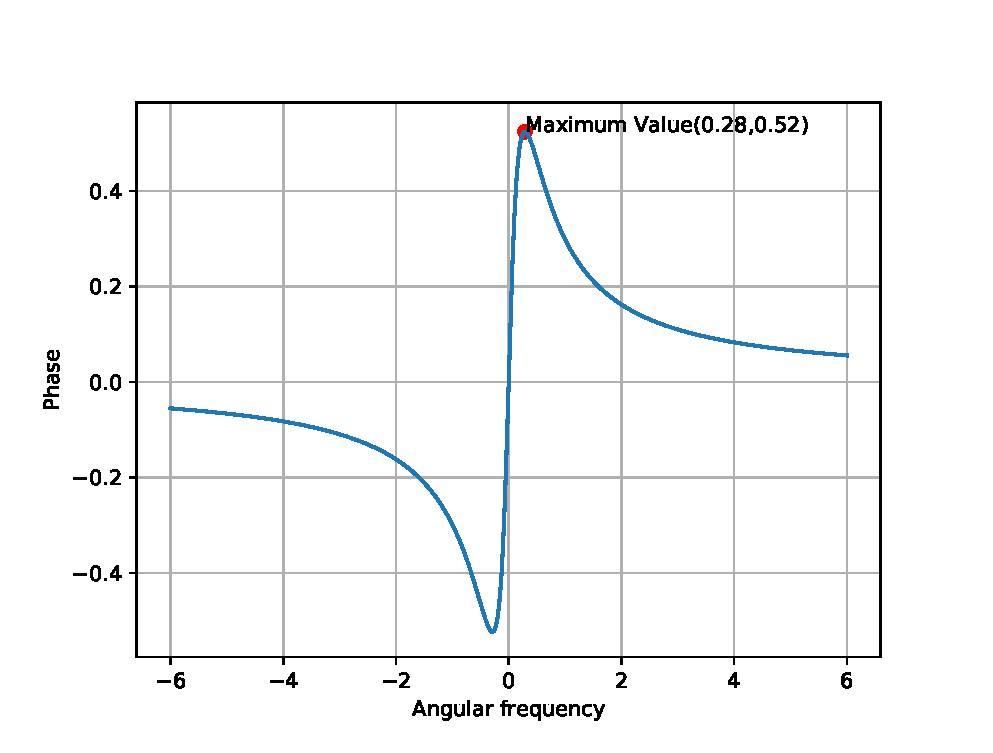
\includegraphics[width=\columnwidth]{./figs/ee18btech11010.eps}
	\caption{}
	\label{fig:ee18btech11010}
\end{figure}
 
\textbf{Applications:}\\ \\
\begin{enumerate}
  \item Phase lead Compensators can be used as High pass filters,Differentiators.
  \item They are used to reduce steady state errors. 
  \item Increases Phase Margin , relative stability.
\end{enumerate}
\item What is purpose of of a Phase Lead Compensator?
\item Through an example, show how the compensator in Problem \ref{prob:ee18btech11010_comp} can be used in a control system.



\end{enumerate}





\end{document}


